\documentclass[11pt,letterpaper]{article}

%% ── packages ────────────────────────────────────────────────────────────────
\usepackage[margin=1in]{geometry}
\usepackage{booktabs}
\usepackage{graphicx}
\usepackage{amsmath}
\usepackage{caption}
\usepackage{subcaption}
\usepackage[T1]{fontenc}
\usepackage{microtype}
\usepackage{parskip}
\usepackage{array}
\usepackage{xcolor}
\usepackage{colortbl}
\usepackage{multirow}
\usepackage[colorlinks=true,linkcolor=blue,urlcolor=blue]{hyperref}
\usepackage{float}
\definecolor{hilight}{gray}{0.80}   %% professor's gray highlight

%% ── title ───────────────────────────────────────────────────────────────────
\begin{document}

\begin{center}
  {\LARGE \textbf{COMPSCI 589-Final Project}}\\[6pt]
  {\large Spring 2026}\\[4pt]
  Ananya Jha \quad Tanvi Kandepuneni \quad Dhriti Madireddy
\end{center}

\vspace{6pt}



%%─────────────────────────────────────────────────────────────────────────────
\section{Dataset 1: Hand Written Digits Recognition}
%%─────────────────────────────────────────────────────────────────────────────

\subsection{Digits dataset}\label{sec:digits_dataset}

We use the handwritten digit collection from our project CSV (8$\times$8 grayscale images, 64 integer pixel features per sample, labels 0--9). There are 1797 samples in total. The ten digit classes are nearly balanced (Figure~\ref{fig:digits_class_dist}), which is why mean accuracy and weighted F1 track each other closely in the tables below. Figure~\ref{fig:digits_samples} shows random $8 \times 8$ examples per class. The remaining figures in this subsection are taken from our \texttt{digits\_classification.ipynb} notebook: cross-validated learning curves for KNN and Random Forest (Figures~\ref{fig:digits_knn}--\ref{fig:digits_rf}), a Gradient Boosting summary (Figure~\ref{fig:digits_gb}), and a bar chart of the best configuration per model family (Figure~\ref{fig:digits_compare}).

\begin{figure}[H]
    \centering
    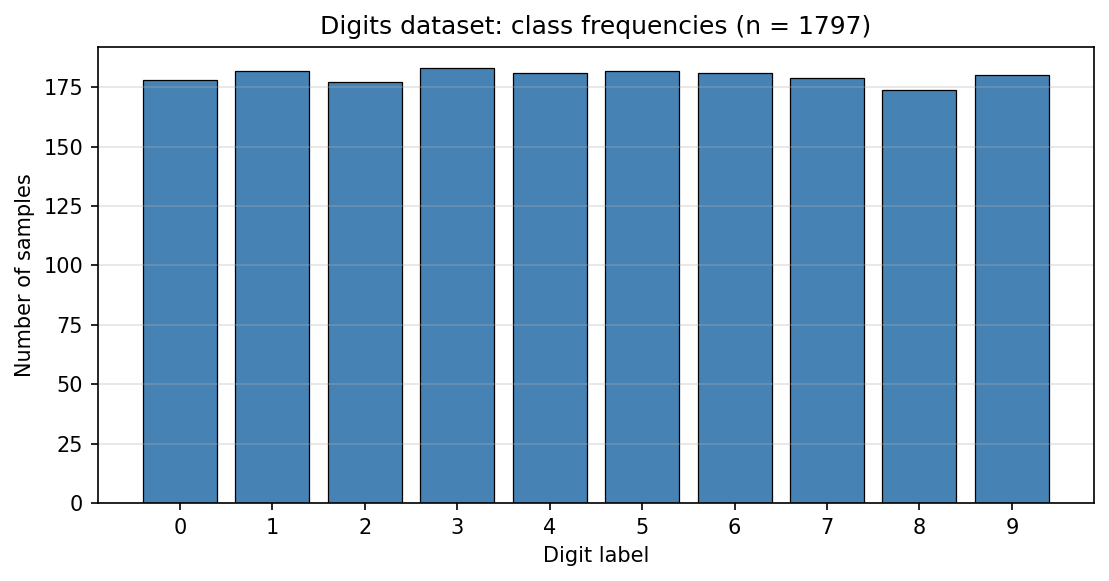
\includegraphics[width=0.75\linewidth]{digits_class_distribution.png}
    \caption{Digits dataset: number of training samples per class (1797 total).}
    \label{fig:digits_class_dist}
\end{figure}

\begin{figure}[H]
    \centering
    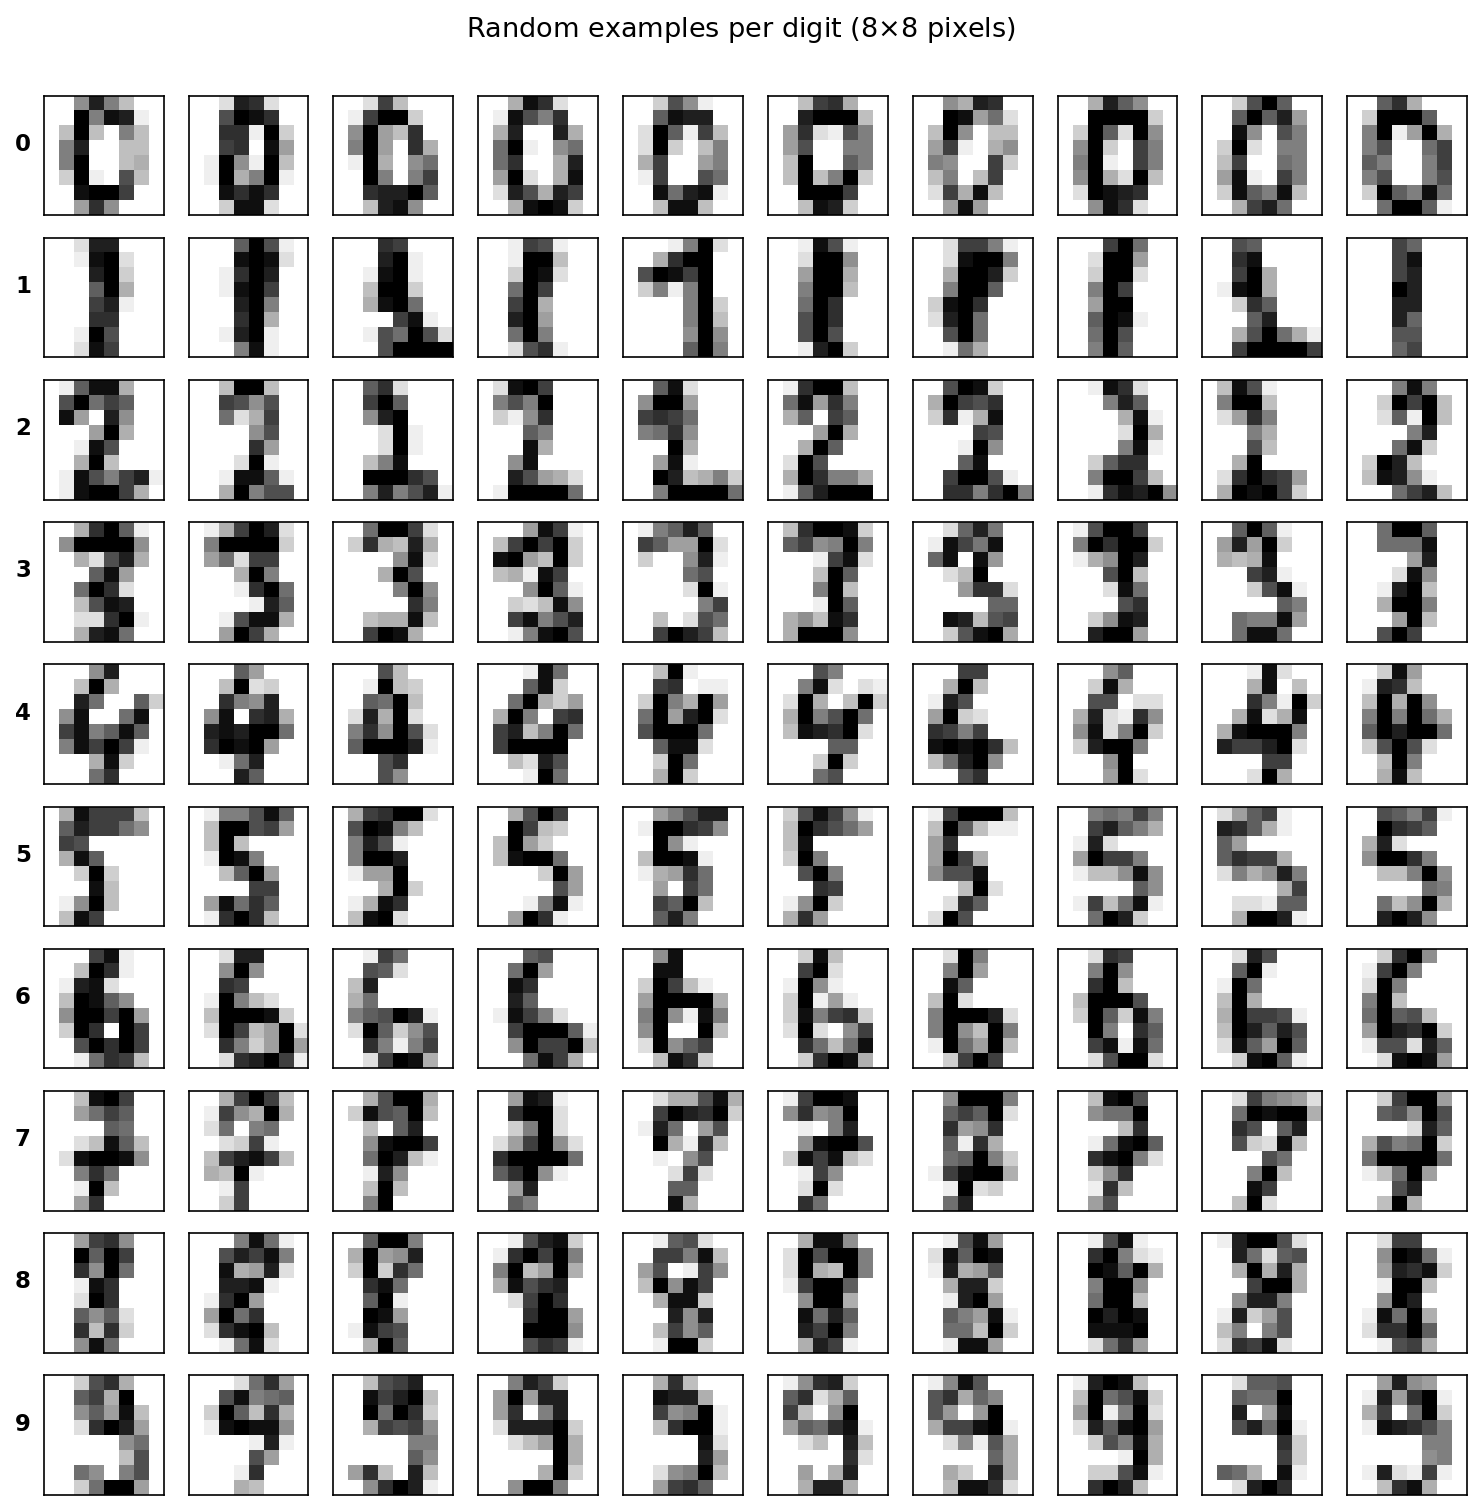
\includegraphics[width=0.88\linewidth]{digits_sample_grid.png}
    \caption{Random examples per digit class ($8 \times 8$ pixels, grayscale).}
    \label{fig:digits_samples}
\end{figure}

\paragraph{Figure~\ref{fig:digits_class_dist} (class balance).}
The bar chart confirms that no digit class dominates: counts per label stay on the same scale, so a single accuracy number remains interpretable next to weighted F1 in our CV tables.

\paragraph{Figure~\ref{fig:digits_samples} (example digits).}
The $10\times 10$ grid illustrates variability in stroke width and slant within each class and shows why pixel-based distances and tree splits can still separate classes despite noisy handwriting.

\begin{figure}[H]
    \centering
    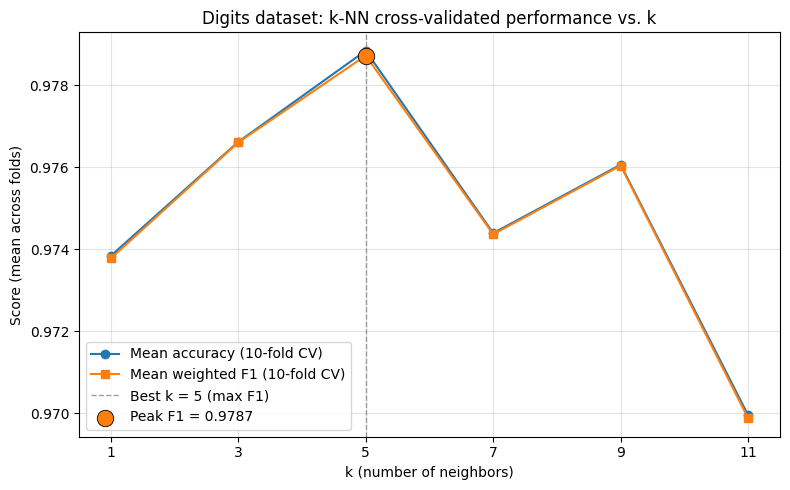
\includegraphics[width=0.62\linewidth]{digits_knn_vs_k.png}
    \caption{KNN on Digits: mean accuracy and weighted F1 vs.\ $k$ (10-fold stratified CV, $z$-score normalised features).}
    \label{fig:digits_knn}
\end{figure}

\begin{figure}[H]
    \centering
    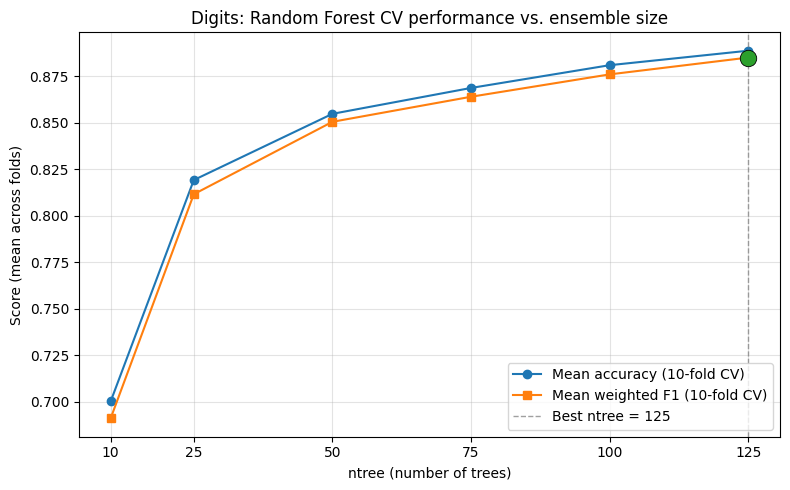
\includegraphics[width=0.62\linewidth]{digits_rf_vs_ntree.png}
    \caption{Random Forest on Digits: mean accuracy and weighted F1 vs.\ \texttt{ntree} (\texttt{max\_depth}${}=12$ per tree).}
    \label{fig:digits_rf}
\end{figure}

\begin{figure}[H]
    \centering
    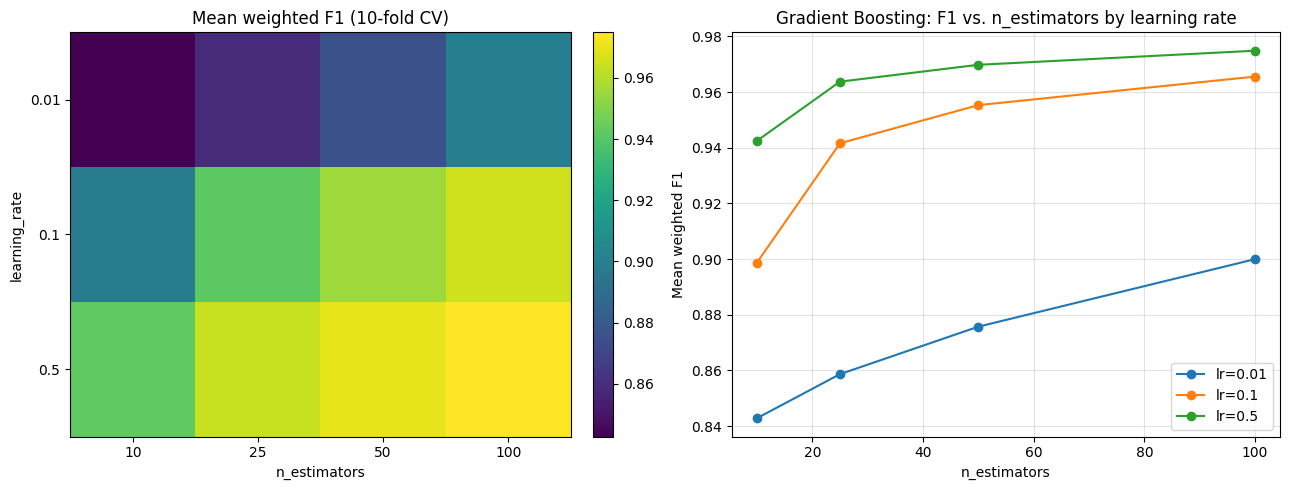
\includegraphics[width=\linewidth]{digits_gb_f1_heatmap_lines.png}
    \caption{Gradient Boosting on Digits: mean weighted F1 heatmap over \texttt{n\_estimators} and \texttt{learning\_rate} (left); mean weighted F1 vs.\ \texttt{n\_estimators} for each learning rate (right).}
    \label{fig:digits_gb}
\end{figure}

\paragraph{Figure~\ref{fig:digits_gb} (Gradient Boosting surfaces).}
The heatmap compresses the $4\times 3$ grid of mean weighted F1 values so the best $(\texttt{n\_estimators},\texttt{learning\_rate})$ combinations pop out as brighter cells; the line plot on the right traces the same metric along \texttt{n\_estimators} for each learning rate and shows that large $\texttt{learning\_rate}$ reaches high F1 with fewer trees but can plateau or dip when too many estimators are stacked.

\begin{figure}[H]
    \centering
    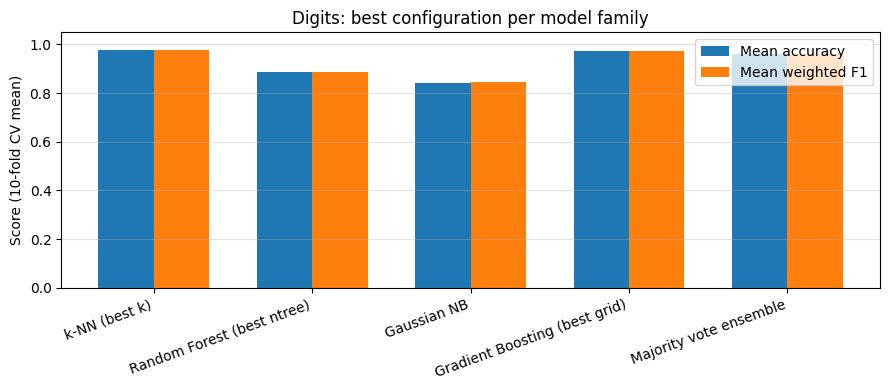
\includegraphics[width=\linewidth]{digits_best_model_comparison.png}
    \caption{Digits: best configuration per model family---mean accuracy vs.\ mean weighted F1 (10-fold CV).}
    \label{fig:digits_compare}
\end{figure}

\paragraph{Figure~\ref{fig:digits_compare} (best model per family).}
Paired accuracy and weighted F1 bars summarise the winning KNN, depth-capped Random Forest, default GNB, best Gradient Boosting configuration, and the three-way majority vote: KNN and GB are tallest, the ensemble sits between them, and RF is pulled down by the depth limit noted above.

\subsection{Algorithm Selection and Justification}

\paragraph{k-Nearest Neighbours (KNN).}
We used k-NN as a simple and intuitive baseline model. Our main idea is that
digits with similar pixel patterns should be close to each other in the
64-dimensional feature space. Since the data was already normalized,
Euclidean distance works well as a similarity measure. $k$ is the main parameter which controls how many neighbouring points are used for prediction. We tested various values of $k$ to study the bias--variance trade-off.

\paragraph{Random Forest (RF).}
Random Forest uses/combines multiple decision trees and makes predictions using majority voting across the trees. This helps reduce overfitting and works well for multi class classification.
The main hyperparameter explored was the number of trees (\texttt{ntree}). Since our Python implementation of decision trees can
grow very deep on continuous pixel values, a limit of $\texttt{max\_depth}=12$ was added to keep the training and 10-fold cross
validation runtime manageable. This limitation is important to consider when
analyzing the RF results.

\paragraph{Gaussian Naive Bayes (GNB) (extra credit).}
We used Gaussian Naive Bayes as a fast probabilistic baseline for
continuous-valued features. GNB assumes the features are independent and they follow a Gaussian distribution. This assumption is not fully true for image pixels because nearby pixels are often correlated. However, GNB is a good baseline for
comparison. No hyperparameter tuning was done for this model.

\paragraph{Gradient Boosting (GB) (extra credit).}
Gradient Boosting is an ensemble method that builds trees sequentially. Each new tree tries to correct the mistakes made by the previous ones. Multiple
hyperparameter combinations were tested using different values of
$\texttt{n\_estimators} \in \{10,25,50,100\}$ and
$\texttt{learning\_rate} \in \{0.01,0.1,0.5\}$. In total, twelve
configurations were evaluated.

\paragraph{Majority-vote Ensemble (extra credit).}
An ensemble model was also created by combining the best-performing KNN
model, the best-performing Random Forest model, and GNB.We made final predictions using majority voting across the three classifiers on the same
stratified folds.

\subsection{Hyperparameter Search}

All results are means over stratified 10-fold cross-validation
(\texttt{random\_state=42}).

\begin{table}[H]
\centering
\caption{KNN on Digits: mean accuracy and weighted F1 vs.\ $k$
         (10-fold stratified CV, $z$-score normalised).}
\label{tab:d1_knn}
\begin{tabular}{@{}ccc@{}}
\toprule
$k$ & Accuracy & Weighted F1 \\
\midrule
1  & 0.9738 & 0.9738 \\
3  & 0.9766 & 0.9766 \\
\rowcolor{hilight}
\textbf{5}  & \textbf{0.9788} & \textbf{0.9787} \\
7  & 0.9744 & 0.9744 \\
9  & 0.9761 & 0.9760 \\
11 & 0.9700 & 0.9699 \\
\bottomrule
\end{tabular}
\end{table}

\begin{table}[H]
\centering
\caption{Random Forest on Digits: mean accuracy and weighted F1 vs.\
         \texttt{ntree} (\texttt{max\_depth}=12 per tree).}
\label{tab:d1_rf}
\begin{tabular}{@{}ccc@{}}
\toprule
\texttt{ntree} & Accuracy & Weighted F1 \\
\midrule
10  & 0.7001 & 0.6910 \\
25  & 0.8191 & 0.8115 \\
50  & 0.8547 & 0.8505 \\
75  & 0.8687 & 0.8639 \\
100 & 0.8809 & 0.8760 \\
\rowcolor{hilight}
\textbf{125} & \textbf{0.8887} & \textbf{0.8850} \\
\bottomrule
\end{tabular}
\end{table}

\begin{table}[H]
\centering
\caption{Gradient Boosting on Digits: 12 hyperparameter configurations.}
\label{tab:d1_gb}
\begin{tabular}{@{}cccc@{}}
\toprule
\texttt{n\_estimators} & \texttt{learning\_rate}
  & Accuracy & Weighted F1 \\
\midrule
10  & 0.01 & 0.8442 & 0.8428 \\
10  & 0.10 & 0.8987 & 0.8987 \\
10  & 0.50 & 0.9427 & 0.9425 \\
25  & 0.01 & 0.8592 & 0.8586 \\
25  & 0.10 & 0.9416 & 0.9416 \\
25  & 0.50 & 0.9638 & 0.9637 \\
50  & 0.01 & 0.8759 & 0.8757 \\
50  & 0.10 & 0.9555 & 0.9553 \\
50  & 0.50 & 0.9699 & 0.9698 \\
100 & 0.01 & 0.8998 & 0.9000 \\
100 & 0.10 & 0.9655 & 0.9655 \\
\rowcolor{hilight}
\textbf{100} & \textbf{0.50} & \textbf{0.9750} & \textbf{0.9748} \\
\bottomrule
\end{tabular}
\end{table}

\noindent Gaussian NB (default hyperparameters):
accuracy $= 0.8425$, weighted F1 $= 0.8439$.\\
Majority-vote ensemble ($k=5$, \texttt{ntree}$=125$, GNB):
accuracy $= 0.9616$, weighted F1 $= 0.9616$.

\subsection{Learning Curves}

Figure~\ref{fig:digits_knn} and Figure~\ref{fig:digits_rf} (Section~\ref{sec:digits_dataset}) show the KNN and Random Forest curves; Figure~\ref{fig:digits_gb} summarises Gradient Boosting over the full grid. Figure~\ref{fig:digits_compare} places all best-tuned models side by side.

\paragraph{Figure~\ref{fig:digits_knn} (KNN vs.\ $k$).}
For us the best performance is when $k=5$. When $k=1$ the model is very
sensitive to noise and can overfit the training data. Using $k=5$ helps
smooth out noisy neighbours while still keeping similar digits close
together. For large $k$, the neighbourhood starts including
different-looking digits and this leads to misclassification which reduces the accuracy. Accuracy and
weighted F1 remain almost identical across all values of $k$. This is
because the dataset is nearly perfectly balanced across the ten classes.

\paragraph{Figure~\ref{fig:digits_rf} (RF vs.\ \texttt{ntree}).}
The Random Forest results improve as the number of trees increases. Accuracy
starts around 0.70 at $\texttt{ntree}=10$ and reaches about 0.89 at
$\texttt{ntree}=125$. The model still does not appear to fully saturate.
However, RF performs much worse than KNN overall. One main reason is the
depth limit of $\texttt{max\_depth}=12$. The trees cannot grow deep enough
to learn detailed pixel boundaries in the 64-dimensional feature space.
Without this depth cap, training became extremely slow, sometimes taking
more than an hour per fold. This limitation is important when interpreting
the RF results.

\subsection{Discussion}

KNN with $k=5$ achieved the best accuracy of 0.9788 on the Digits dataset.
It slightly outperformed Gradient Boosting, which achieved 0.9750. This
shows that instance-based learning works very well when similar samples
naturally cluster together in feature space. The depth-capped Random Forest
had the weakest performance among the main models. The majority-vote
ensemble also performed worse than KNN alone. This is likely because the
weaker RF and GNB models reduced the overall ensemble quality when they
made incorrect predictions.

%%─────────────────────────────────────────────────────────────────────────────
\section{Dataset 2: Oxford Parkinson's Disease Detection}
%%─────────────────────────────────────────────────────────────────────────────

\subsection{Parkinson's dataset and notebook figures}\label{sec:parkinsons_figures}

We use the Oxford Parkinson's speech dataset from our project CSV: $195$ samples, $22$ voice-related features, and a binary label (1 = Parkinson's, 0 = healthy). The minority class is healthy controls; the majority class is Parkinson's diagnoses, so accuracy alone can be misleading and weighted F1 matters. Figures~\ref{fig:park_knn}--\ref{fig:park_compare} reproduce all plots saved from \texttt{parkinsons\_classification.ipynb}: KNN and Random Forest learning curves over the hyperparameter grids, a two-panel Gradient Boosting summary (heatmap of mean weighted F1 over \texttt{n\_estimators} $\times$ \texttt{learning\_rate} plus F1 vs.\ \texttt{n\_estimators} by learning rate), and a bar chart of each model family at its best configuration (10-fold stratified CV means).

\begin{figure}[H]
        \centering
        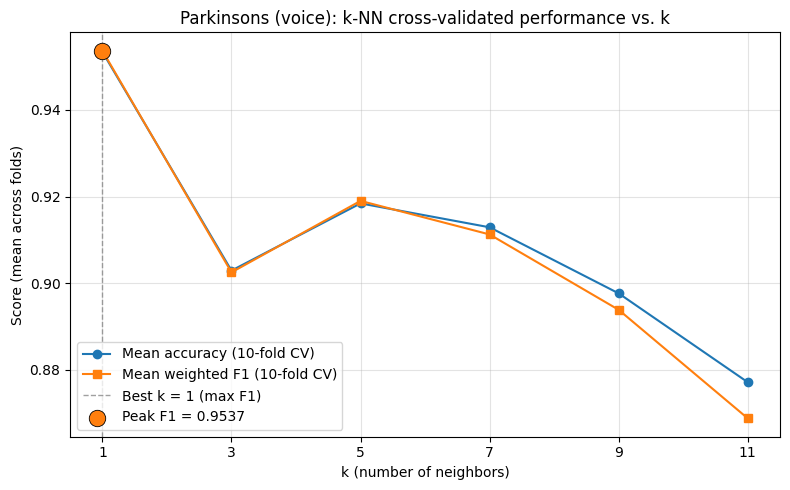
\includegraphics[width=0.62\linewidth]{parkinsons_knn_vs_k.png}
        \caption{Parkinson's: KNN mean accuracy and weighted F1 vs.\ $k$.}
        \label{fig:park_knn}
\end{figure}

\begin{figure}[H]
    \centering
    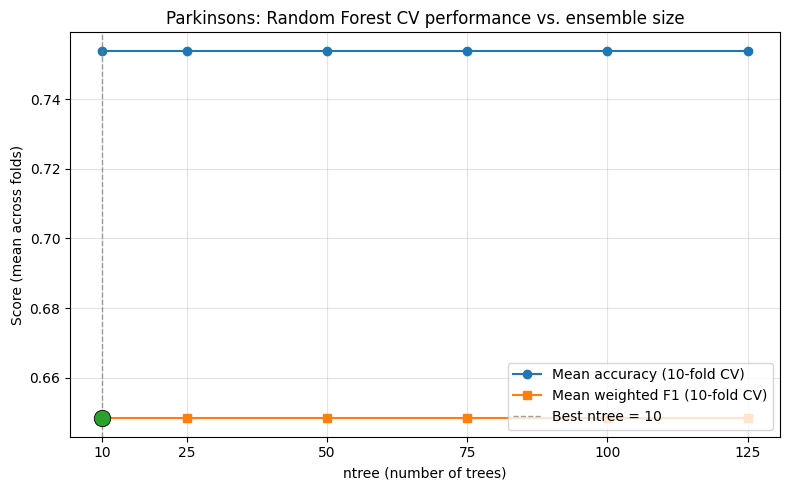
\includegraphics[width=0.62\linewidth]{parkinsons_rf_vs_ntree.png}
    \caption{Parkinson's: Random Forest mean accuracy and weighted F1 vs.\ \texttt{ntree} (\texttt{max\_depth}${}=12$).}
    \label{fig:park_rf}
\end{figure}

\begin{figure}[H]
    \centering
    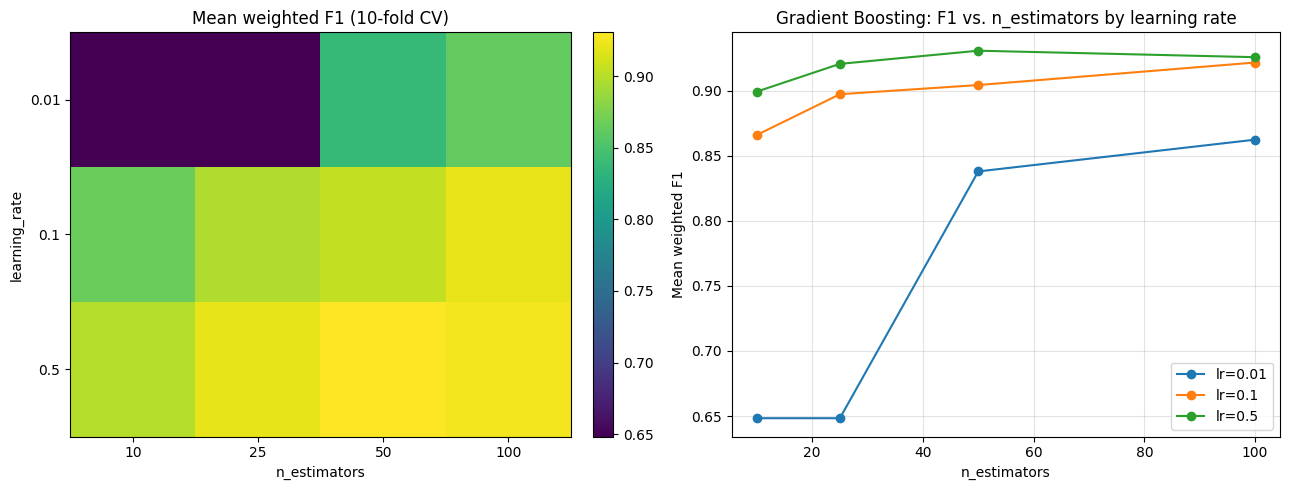
\includegraphics[width=\linewidth]{parkinsons_gb_f1_heatmap_lines.png}
    \caption{Parkinson's: Gradient Boosting---mean weighted F1 heatmap (left); mean weighted F1 vs.\ \texttt{n\_estimators} by \texttt{learning\_rate} (right).}
    \label{fig:park_gb}
\end{figure}

\begin{figure}[H]
    \centering
    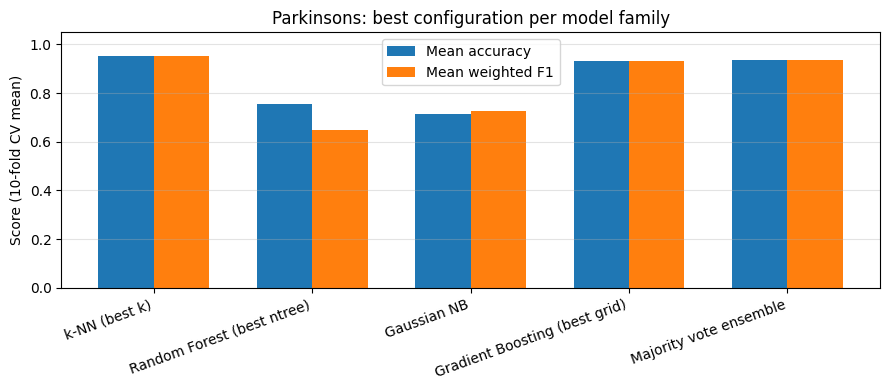
\includegraphics[width=\linewidth]{parkinsons_best_model_comparison.png}
    \caption{Parkinson's: best configuration per model family---mean accuracy vs.\ mean weighted F1 (10-fold CV).}
    \label{fig:park_compare}
\end{figure}

\paragraph{Discussion of Figures~\ref{fig:park_knn}--\ref{fig:park_compare}.}
Figure~\ref{fig:park_knn} plots the same KNN grid as Table~\ref{tab:d2_knn}; Figure~\ref{fig:park_rf} shows RF flatlining at the majority-class accuracy; Figure~\ref{fig:park_gb} combines the F1 heatmap with traces of F1 over \texttt{n\_estimators} for each \texttt{learning\_rate}; Figure~\ref{fig:park_compare} condenses the best KNN, RF, GNB, GB, and ensemble scores into one bar chart for quick comparison with Tables~\ref{tab:d2_knn}--\ref{tab:d2_gb}.
Detailed interpretation follows in the Learning Curves subsection below.

\subsection{Algorithm Selection and Justification}

\paragraph{KNN}
We chose KNN because the measurements form a continuous feature space. Here we can use Euclidean distance as it capture similarity between samples.
Since the dataset is small, and also that the learning is instance based methods like KNN work
well and do not require heavy parameter estimation.

\paragraph{Random Forest}
Random Forest was used to reduce the variance of individual decision trees
through bagging and majority voting. However, the dataset is both small and
imbalanced, which creates challenges for the pure-Python implementation.
Without class balancing, the trees tend to favour the majority class during
splits, especially in uncertain regions. This can reduce the overall
performance of the ensemble.

\paragraph{Gaussian NB and Gradient Boosting - extra credit.}
Gaussian Naive Bayes and Gradient Boosting were included for the same reasons
as in Dataset~1. Gradient Boosting is especially useful for imbalanced data
because each new tree focuses more on previously misclassified examples,
including minority-class samples.

\subsection{Hyperparameter Search}

\begin{table}[H]
\centering
\caption{KNN on Parkinson's: accuracy and weighted F1 vs.\ $k$.}
\label{tab:d2_knn}
\begin{tabular}{@{}ccc@{}}
\toprule
$k$ & Accuracy & Weighted F1 \\
\midrule
\rowcolor{hilight}
\textbf{1}  & \textbf{0.9534} & \textbf{0.9537} \\
3  & 0.9029 & 0.9025 \\
5  & 0.9184 & 0.9190 \\
7  & 0.9129 & 0.9112 \\
9  & 0.8976 & 0.8938 \\
11 & 0.8771 & 0.8688 \\
\bottomrule
\end{tabular}
\end{table}

\begin{table}[H]
\centering
\caption{Random Forest on Parkinson's: all configurations degenerate to
         majority-class prediction (\texttt{max\_depth}=12).}
\label{tab:d2_rf}
\begin{tabular}{@{}ccc@{}}
\toprule
\texttt{ntree} & Accuracy & Weighted F1 \\
\midrule
10  & 0.7539 & 0.6483 \\
25  & 0.7539 & 0.6483 \\
50  & 0.7539 & 0.6483 \\
75  & 0.7539 & 0.6483 \\
100 & 0.7539 & 0.6483 \\
125 & 0.7539 & 0.6483 \\
\bottomrule
\end{tabular}
\end{table}

\begin{table}[H]
\centering
\caption{Gradient Boosting on Parkinson's: 12 configurations.}
\label{tab:d2_gb}
\begin{tabular}{@{}cccc@{}}
\toprule
\texttt{n\_estimators} & \texttt{learning\_rate}
  & Accuracy & Weighted F1 \\
\midrule
10  & 0.01 & 0.7539 & 0.6483 \\
10  & 0.10 & 0.8761 & 0.8659 \\
10  & 0.50 & 0.9071 & 0.8992 \\
25  & 0.01 & 0.7539 & 0.6483 \\
25  & 0.10 & 0.9016 & 0.8972 \\
25  & 0.50 & 0.9224 & 0.9205 \\
50  & 0.01 & 0.8555 & 0.8379 \\
50  & 0.10 & 0.9066 & 0.9042 \\
\rowcolor{hilight}
\textbf{50} & \textbf{0.50} & \textbf{0.9326} & \textbf{0.9306} \\
100 & 0.01 & 0.8761 & 0.8623 \\
100 & 0.10 & 0.9221 & 0.9215 \\
100 & 0.50 & 0.9274 & 0.9256 \\
\bottomrule
\end{tabular}
\end{table}

\noindent Gaussian NB:
accuracy $= 0.7132$, weighted F1 $= 0.7283$.\\
Majority-vote ensemble ($k=1$, \texttt{ntree}$=10$, GNB):
accuracy $= 0.9379$, weighted F1 $= 0.9367$.

\subsection{Learning Curves}

The KNN, Random Forest, Gradient Boosting, and model-comparison plots appear in Section~\ref{sec:parkinsons_figures} as Figures~\ref{fig:park_knn}--\ref{fig:park_compare}.

\paragraph{Figure~\ref{fig:park_knn} (KNN vs.\ $k$).}
Unlike the Digits dataset, the best performance is achieved at $k=1$.
Accuracy reaches 0.9534 and then decreases steadily as $k$ increases.
This happens because the dataset is small and highly imbalanced. There are
many more Parkinson's samples than healthy samples. With a small value of
$k$, healthy samples are more likely to stay close to other healthy samples
in feature space. The strong performance at $k=1$ suggests that the voice
features are highly discriminative. As $k$ becomes larger, neighbourhoods
contain more Parkinson's samples, causing predictions to bias toward the
majority class. This lowers healthy-class recall and reduces both accuracy
and F1 score.

\paragraph{Figure~\ref{fig:park_rf} (RF vs.\ \texttt{ntree}).}
Accuracy and weighted F1 are flat across all numbers of trees: both stay near $0.754$ and $0.648$ respectively. This matches majority-class dominance (predicting Parkinson's for almost every hold-out fold). Random Forest does not improve with more trees because the depth-capped, unbalanced splits already collapse to the majority label.

\paragraph{Figure~\ref{fig:park_gb} (Gradient Boosting).}
Different learning rates show different behaviours. At
$\texttt{learning\_rate}=0.01$, the model improves very slowly and needs many
estimators to achieve reasonable performance. At
$\texttt{learning\_rate}=0.1$, the model converges much faster and continues
to improve steadily as the number of estimators increases. At
$\texttt{learning\_rate}=0.5$, the model learns very quickly and achieves
high accuracy even with a small number of estimators. However, performance
slightly decreases after too many estimators are added, which suggests mild
overfitting.

\paragraph{Figure~\ref{fig:park_compare} (best model per family).}
The grouped bars summarise the best mean CV accuracy and weighted F1 for KNN, Random Forest, Gaussian NB, Gradient Boosting, and the majority-vote ensemble. KNN and Gradient Boosting reach the highest bars; Random Forest and Gaussian NB sit lower, consistent with Tables~\ref{tab:d2_knn}--\ref{tab:d2_gb}.

\subsection{Discussion}

KNN with $k=1$ achieved the best performance on this dataset with an
accuracy of 0.9534. The Random Forest model performed poorly, reaching
0.7539 accuracy for all values of \texttt{ntree}. This is almost exactly
equal to the majority-class ratio of the dataset. The weighted F1 score also
shows that RF mainly predicted the Parkinson's class for nearly every
sample. This highlights a limitation of the implementation on small,
imbalanced datasets without class balancing. Gradient Boosting performed
much better because boosting places more focus on previously misclassified
samples, including minority-class examples. GNB also performed poorly,
likely because many voice features are strongly correlated and violate the
independence assumption. The majority-vote ensemble performed between KNN
and Gradient Boosting overall.
%%─────────────────────────────────────────────────────────────────────────────
\section{Dataset 3: Rice Grains}
%%─────────────────────────────────────────────────────────────────────────────

\noindent\textbf{Dataset summary (from \texttt{rice\_experiment.py}).}
The Rice Cammeo vs.\ Osmancik dataset has $3810$ samples and $7$ numerical features per grain.
The class counts are Cammeo $=1630$ and Osmancik $=2180$ (Osmancik is the majority class).
All metrics below are means from stratified 10-fold cross-validation with \texttt{seed=42},
matching the console summary and \texttt{figures/rice\_evaluation\_summary.csv}.

\subsection{Algorithm Selection and Justification}

\paragraph{KNN.}
All seven features are continuous numerical values, so Euclidean distance works well after feature normalization. Also, KNN also does not make strong
assumptions about the data. We did a Stratified 10-fold cross-validation from scratch using the custom
\texttt{stratified\_kfold} function in \texttt{rice\_experiment.py}.
Accuracy and binary F1 score were also calculated using custom
\texttt{numpy}-based functions.

\paragraph{Neural Network}
We used a feedforward neural network with sigmoid activations and batch gradient
descent learn non-linear relationships between the features.
The dataset has 3,810 samples and 7 input features, so a small single hidden layer network can be trained without too much overfitting.
The output layer uses a single sigmoid neuron for binary classification, and binary cross-entropy as loss function.

\subsection{Hyperparameter Search}

\begin{table}[H]
\centering
\caption{KNN on Rice Grains: accuracy and binary F1 vs.\ $k$
         (10-fold stratified CV, normalised).}
\label{tab:d3_knn}
\begin{tabular}{@{}ccc@{}}
\toprule
$k$ & Accuracy & F1-Score \\
\midrule
1  & 0.8856 & 0.8995 \\
3  & 0.9060 & 0.9180 \\
5  & 0.9178 & 0.9283 \\
7  & 0.9228 & 0.9326 \\
9  & 0.9231 & 0.9330 \\
11 & 0.9228 & 0.9328 \\
15 & 0.9252 & 0.9348 \\
\rowcolor{hilight}
\textbf{21} & \textbf{0.9273} & \textbf{0.9366} \\
\bottomrule
\end{tabular}
\end{table}

\begin{table}[ht]
\centering
\caption{Neural Network on Rice Grains: 8 configurations
         (10-fold stratified CV, normalised inputs).}
\label{tab:d3_nn}
\begin{tabular}{@{}llcccc@{}}
\toprule
Architecture & LR & $\lambda$ & Iters & Accuracy & F1 \\
\midrule
\rowcolor{hilight}
\textbf{[7,16,1]} & \textbf{0.10} & \textbf{0.000}
  & \textbf{1000} & \textbf{0.9281} & \textbf{0.9372} \\
{[7,32,1]}    & 0.10 & 0.000 & 1000 & 0.9260 & 0.9352 \\
{[7,64,1]}    & 0.05 & 0.000 & 1000 & 0.9262 & 0.9352 \\
{[7,16,8,1]}  & 0.10 & 0.000 & 1000 & 0.9276 & 0.9367 \\
{[7,32,16,1]} & 0.10 & 0.000 & 1000 & 0.9268 & 0.9359 \\
{[7,32,1]}    & 0.10 & 0.010 & 1000 & 0.9260 & 0.9352 \\
{[7,32,1]}    & 0.10 & 0.001 & 2000 & 0.9260 & 0.9352 \\
{[7,16,1]}    & 0.10 & 0.001 & 2000 & 0.9276 & 0.9367 \\
\bottomrule
\end{tabular}
\end{table}

\subsection{Learning Curves}

\begin{figure}[H]
    \centering
    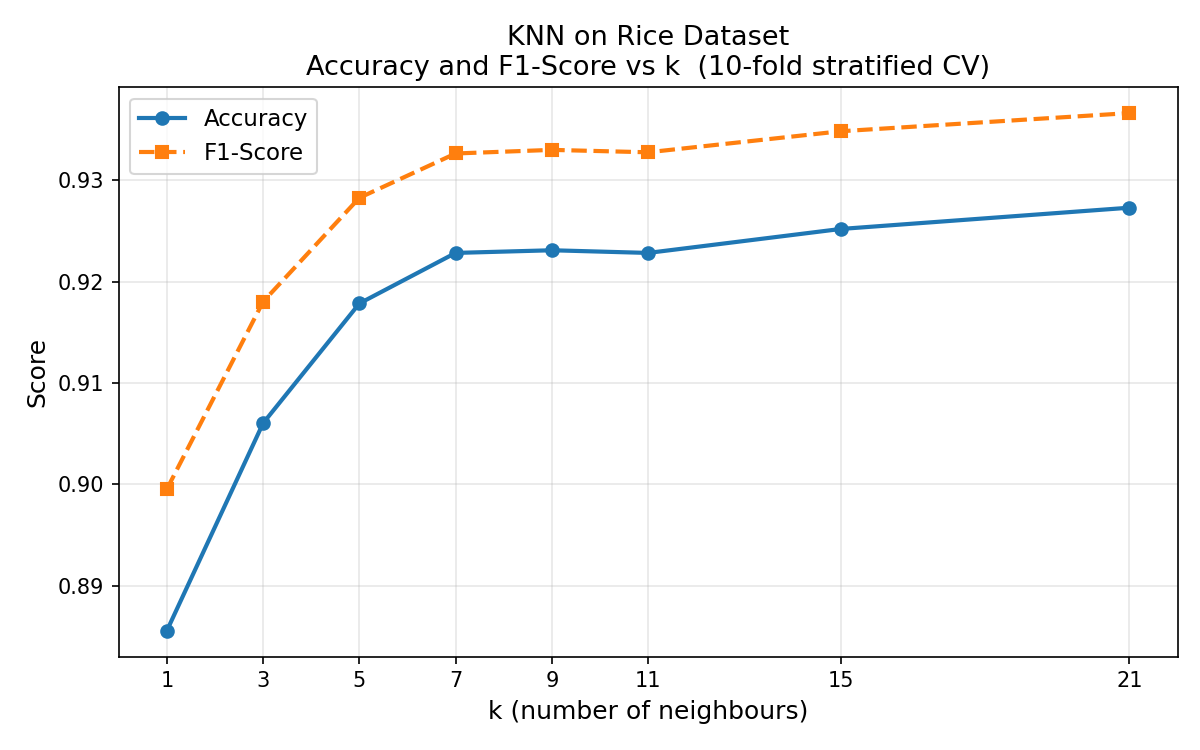
\includegraphics[width=0.55\linewidth]{rice_knn_vs_k.png}
    \caption{Rice: KNN mean accuracy and F1 vs.\ $k$ (same plot as \texttt{figures/rice\_knn\_vs\_k.png}).}
    \label{fig:rice_knn}
\end{figure}

\begin{figure}[H]
    \centering
    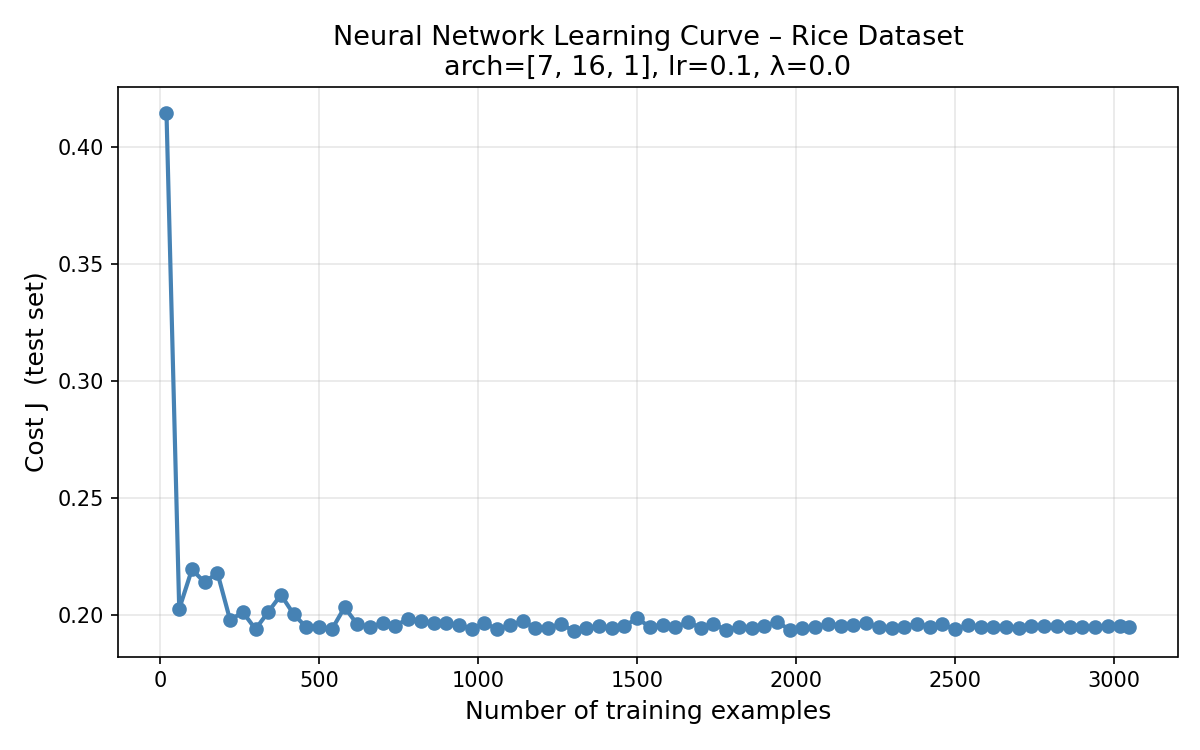
\includegraphics[width=0.55\linewidth]{rice_nn_learning_curve.png}
    \caption{Neural network learning curve: cost $J$ on a held-out test fold vs.\ training-set size (best config \texttt{[7,16,1]}, lr${}=0.10$, $\lambda=0$; 77 points).}
    \label{fig:rice_nn_lc}
\end{figure}
\paragraph{Figure~\ref{fig:rice_knn} (KNN vs.\ $k$).}
as k increases both accuracy and F1 score improve steadily. Accuracy rises
from 0.8856 at $k=1$ to 0.9273 at $k=21$. The improvement is strongest up to
around $k=7$ after this point they start to level. Even with larger values of k the performance doesn't decrease so the optimum k value might be more than 21. By this we can say that boundary between the Cammeo and Osmancik
classes is relatively smooth in the 7-dimensional feature space. The F1 score
is slightly more than accuracy throughout because the Osmancik class is the majority class in the dataset.

\paragraph{Figure~\ref{fig:rice_nn_lc} (Neural Network learning curve).}
We see that the training cost decreases pretty quickly as more training examples are added.
The cost starts around 0.415 with 20 samples and drops to around 0.20 by
around 80 samples. Then after that the curve changes only slightly and becomes
stable near 0.196 after around 500 examples. This shows that the neural
network learns the main class patterns with even small data. The flat
curve at larger dataset sizes show that adding more training data does improve performance by much. The remaining error is likely due to model limitations or overlap between the classes.

\subsection{Discussion}

KNN with $k=21$ and the Neural Network achieved very similar performance, they had accuracies of 0.9273 and 0.9281 respectively. This is probably because the two rice classes are well separated. The neural
network performed best with the smallest tested architecture,
\texttt{[7,16,1]}. Larger and deeper networks did not improve performance, this hints that the classification boundary wasn't complex.
$\ell_2$ regularisation also did not improve results, so overfitting wasn't also much of an issue.

\subsection{Extra Credit Tasks (Rice)}

For Rice, we completed additional extra-credit evaluations with Gaussian NB
(EC1: additional algorithm) and a majority-vote ensemble (EC3). The ensemble
combines KNN, Neural Network, and Gaussian NB predictions using fold-wise
majority voting.

\begin{table}[H]
\centering
\caption{Gaussian Naive Bayes on Rice (EC1): accuracy and binary F1 vs.\ smoothing
  ($10$-fold stratified CV, normalised features).}
\label{tab:d3_gnb}
\begin{tabular}{@{}lcc@{}}
\toprule
Smoothing & Accuracy & F1-Score \\
\midrule
$10^{-12}$ & 0.9168 & 0.9277 \\
$10^{-10}$ & 0.9168 & 0.9277 \\
$10^{-8}$  & 0.9168 & 0.9277 \\
$10^{-6}$  & 0.9168 & 0.9277 \\
$10^{-4}$  & 0.9168 & 0.9277 \\
$10^{-3}$  & 0.9168 & 0.9277 \\
$10^{-2}$  & 0.9173 & 0.9282 \\
\rowcolor{hilight}
\textbf{$10^{-1}$} & \textbf{0.9178} & \textbf{0.9289} \\
\bottomrule
\end{tabular}
\end{table}

\begin{table}[H]
\centering
\caption{Rice (extra credit): best configuration per model family (10-fold stratified CV;
         full-precision means match \texttt{rice\_evaluation\_summary.csv}).}
\label{tab:d3_ec}
\begin{tabular}{@{}lcc@{}}
\toprule
Model & Accuracy & F1-Score \\
\midrule
KNN ($k=21$) & 0.927296588 & 0.936631047 \\
\rowcolor{hilight}
NN (best config) & \textbf{0.928083990} & \textbf{0.937180932} \\
GNB (best smoothing $=10^{-1}$) & 0.917847769 & 0.928876019 \\
Ensemble (3 NNs + 1 KNN, EC3) & 0.927559055 & 0.936652744 \\
\bottomrule
\end{tabular}
\end{table}

\begin{figure}[H]
    \centering
    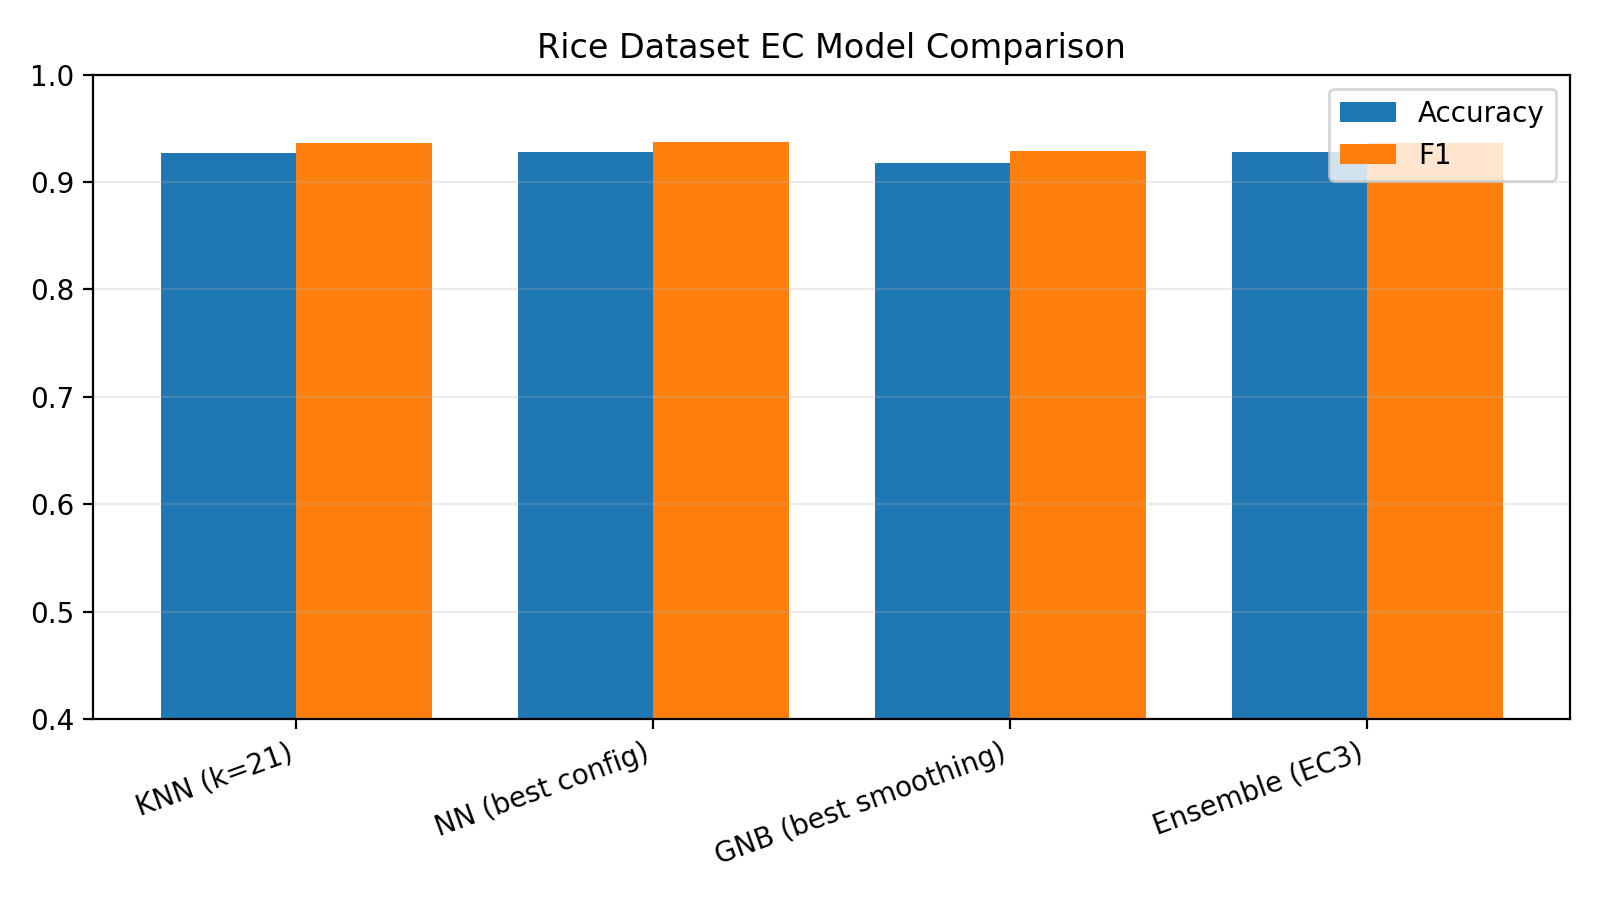
\includegraphics[width=0.72\linewidth]{rice_model_comparison.png}
    \caption{Rice: best KNN, NN, GNB, and ensemble (10-fold CV). The script writes this plot to
             \texttt{figures/rice\_model\_comparison.png}; we also keep an identical copy in the submission folder
             as \texttt{rice\_ec\_model\_comparison.png} so every \texttt{rice\_*.png} artifact is present.}
    \label{fig:rice_model_bar}
\end{figure}

\paragraph{Figure~\ref{fig:rice_model_bar} (best models and ensemble).}
The bar pairs line up with Table~\ref{tab:d3_ec}: NN edges KNN on both metrics, GNB trails, and the ensemble nearly matches the best single models---confirming visually that no single base learner dominates by a large margin on this dataset.

The EC results on Rice are consistent with the main section: all models perform
strongly, and differences are small. Neural Network remains the best single
model, while the ensemble is very close but does not surpass it. Gaussian NB is
weaker because the feature-independence assumption is not fully valid for these
morphological variables; performance is flat for small smoothing values and
only improves once smoothing reaches $10^{-2}$ and $10^{-1}$ (Table~\ref{tab:d3_gnb}).
%%─────────────────────────────────────────────────────────────────────────────
\section{Dataset 4: Credit Approval}
%%─────────────────────────────────────────────────────────────────────────────

\noindent\textbf{Dataset summary (from \texttt{credit\_experiment.py}).}
The Credit Approval dataset has $653$ instances and $15$ fields: $10$ categorical and $5$
numerical features after loading the raw attributes. The binary label counts are
rejected (class~0) $=357$ and approved (class~1) $=296$.
Full hyperparameter grids, plots, and the EC summary table are written to \texttt{figures/}
(e.g.\ \texttt{credit\_evaluation\_table.csv} and \texttt{credit\_extra\_credit\_writeup.md}).

\subsection{Algorithm Selection and Justification}

\paragraph{Decision Tree.}
The decision tree uses information gain to split the data. this really works well
for the 9 categorical features in our dataset. The 5 numerical features
were divided into four bins using only the training data so there would be
no data leakage. This converts the numerical features into discrete values
that the tree can easilyy handle. The main hyperparameter is the early stop
threshold. This basically  stops the tree from splitting more when one class becomes
dominant in a node. We tested seven different threshold values.

\paragraph{KNN.}
For KNN the categorical features (9 features) were one-hot encoded using only the
categories from the training folds. The 5 numerical features were
normalised using $z$-score. This converts each sample into a numerical vector that can be used with Euclidean distance. We tested
different values of $k$. We also didn't use a neural network because
the dataset is kind of small as it only has 653 samples, so KNN made more sense.

\subsection{Hyperparameter Search}

\begin{table}[ht]
\centering
\caption{Decision Tree on Credit Approval: accuracy and binary F1 vs.\
         early-stop threshold (numerical features quartile-binned,
         10-fold stratified CV).}
\label{tab:d4_dt}
\begin{tabular}{@{}ccc@{}}
\toprule
Early-Stop Threshold & Accuracy & F1-Score \\
\midrule
None (full tree) & 0.8255 & 0.8064 \\
\rowcolor{hilight}
\textbf{0.60} & \textbf{0.8638} & \textbf{0.8623} \\
0.65 & 0.8638 & 0.8623 \\
0.70 & 0.8638 & 0.8623 \\
0.75 & 0.8638 & 0.8623 \\
0.80 & 0.8529 & 0.8394 \\
0.85 & 0.8560 & 0.8395 \\
\bottomrule
\end{tabular}
\end{table}

\begin{table}[ht]
\centering
\caption{KNN on Credit Approval: accuracy and binary F1 vs.\ $k$
         (one-hot encoded, $z$-score normalised, 10-fold stratified CV).}
\label{tab:d4_knn}
\begin{tabular}{@{}ccc@{}}
\toprule
$k$ & Accuracy & F1-Score \\
\midrule
1  & 0.7779 & 0.7491 \\
\rowcolor{hilight}
\textbf{3}  & \textbf{0.8133} & \textbf{0.7848} \\
5  & 0.8086 & 0.7761 \\
7  & 0.8038 & 0.7639 \\
9  & 0.8117 & 0.7697 \\
11 & 0.8117 & 0.7688 \\
15 & 0.8024 & 0.7493 \\
21 & 0.7961 & 0.7359 \\
\bottomrule
\end{tabular}
\end{table}

\subsection{Learning Curves}

\begin{figure}[H]
    \centering
    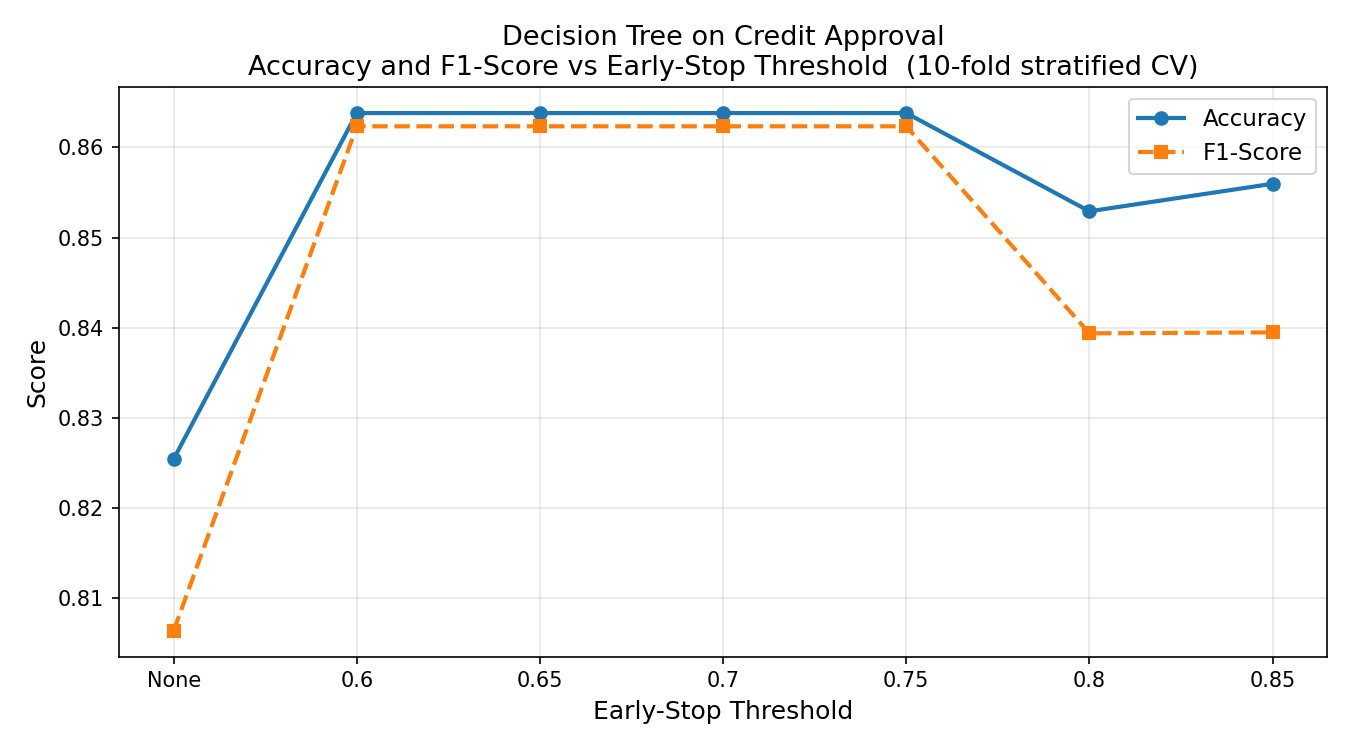
\includegraphics[width=0.52\linewidth]{credit_dt_threshold.png}
    \caption{Credit: Decision Tree mean accuracy and F1 vs.\ early-stop threshold (same plot as \texttt{figures/credit\_dt\_threshold.png}).}
    \label{fig:credit_dt}
\end{figure}

\begin{figure}[H]
    \centering
    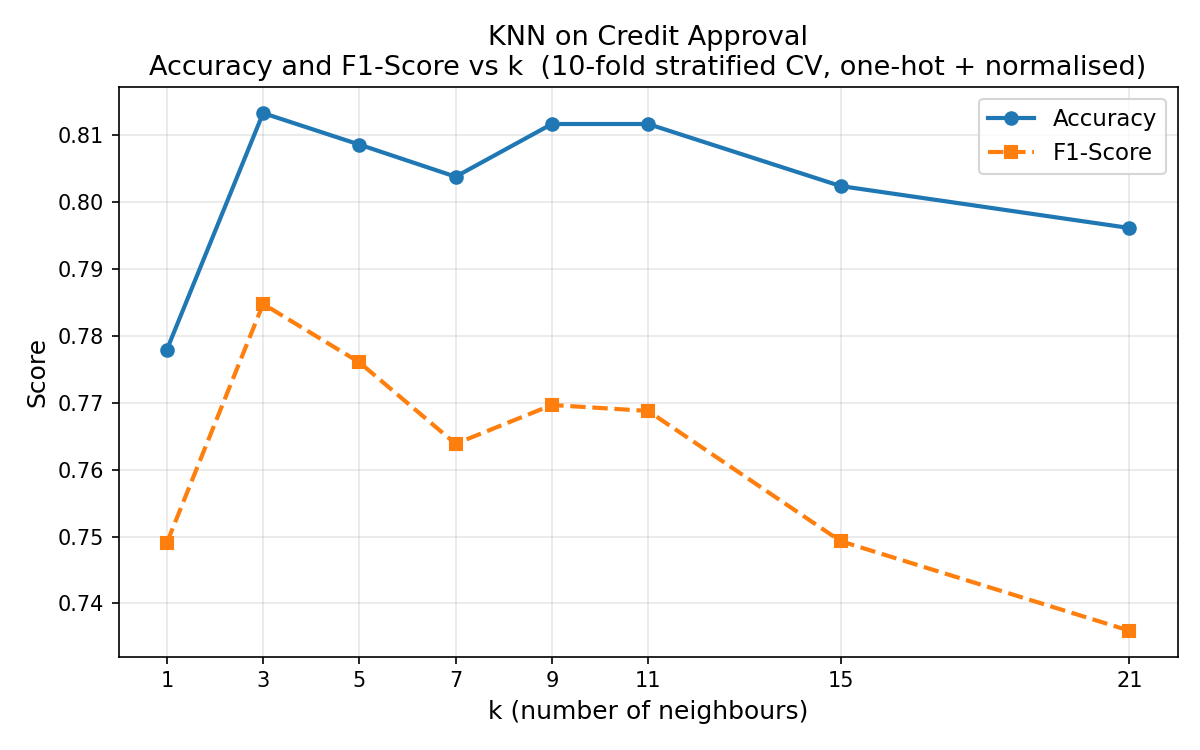
\includegraphics[width=0.52\linewidth]{credit_knn_vs_k.png}
    \caption{Credit: KNN mean accuracy and F1 vs.\ $k$ (one-hot + normalised; \texttt{figures/credit\_knn\_vs\_k.png}).}
    \label{fig:credit_knn}
\end{figure}
\paragraph{Figure~\ref{fig:credit_dt} (Decision Tree vs.\ threshold).}
We see three different patterns in our Decision Tree results. First the fully grown
tree without any stopping threshold gives the worst performance with accuracy 0.8255 and F1 score 0.8064. So the model is
overfitting on the training data. The lower F1 score also shows that the minority approved class is affected more by overfitting.

Second, thresholds from 0.60 to 0.75 all give the same results. This means that
the tree ends up stopping at the same places, so the overall tree structure
does not really much in this range.

Finally, thresholds of 0.80 and 0.85 reduce performance. This strong thresholds probably remove too much useful information, especially for the minority class. Because of this, the F1 score drops more than the accuracy.

\paragraph{Figure~\ref{fig:credit_knn} (KNN vs.\ $k$).}
KNN performs best at $k=3$. Accuracy and F1 both decrease as $k$ increases. When $k=1$ predictions are noisy because the one-hot encoded feature
space is sparse. When $k$ is larger, neighbourhoods contain more majority class samples, this can create bias in predictions toward rejected loans.
Although here for us the accuracy decreases slowly,  F1 drops more sharply because minority-class
recall becomes worse. The growing gap between accuracy and F1 suggests that
the classifier becomes increasingly biased toward the majority class as $k$
increases.

\subsection{Discussion}

The Decision Tree performs better than KNN on this dataset(has higher accuracy and F1). This is probably because the dataset contains many
categorical features, which decision trees handle naturally through feature
splits. KNN on the other hand depends on the Euclidean distance in the one-hot encoded
space. This is less effective for categorical attributes that are unordered. Also the Decision Tree performs consistently well across
thresholds from 0.60 to 0.75. This means that the model is robust or unchanged to small threshold changes.

\subsection{Extra Credit Tasks (Credit)}

For Credit Approval, we also completed EC1 (Gaussian NB baseline) and EC3
(heterogeneous ensemble with Decision Tree + KNN + Gaussian NB + Random
Forest). Results below are from stratified 10-fold CV.

\begin{table}[H]
\centering
\caption{Gaussian Naive Bayes on Credit Approval (EC1): accuracy and binary F1 vs.\
  \texttt{var\_smoothing} (one-hot + normalised, 10-fold stratified CV).}
\label{tab:d4_gnb}
\begin{tabular}{@{}lcc@{}}
\toprule
\texttt{var\_smoothing} & Accuracy & F1-Score \\
\midrule
$10^{-12}$ & 0.6248 & 0.3197 \\
$10^{-11}$ & 0.6326 & 0.3419 \\
$10^{-10}$ & 0.6434 & 0.3768 \\
$10^{-9}$  & 0.6662 & 0.4369 \\
$10^{-8}$  & 0.6723 & 0.4558 \\
\rowcolor{hilight}
\textbf{$10^{-7}$}  & \textbf{0.6723} & \textbf{0.4643} \\
$10^{-6}$  & 0.6723 & 0.4643 \\
\bottomrule
\end{tabular}
\end{table}

\begin{figure}[H]
    \centering
    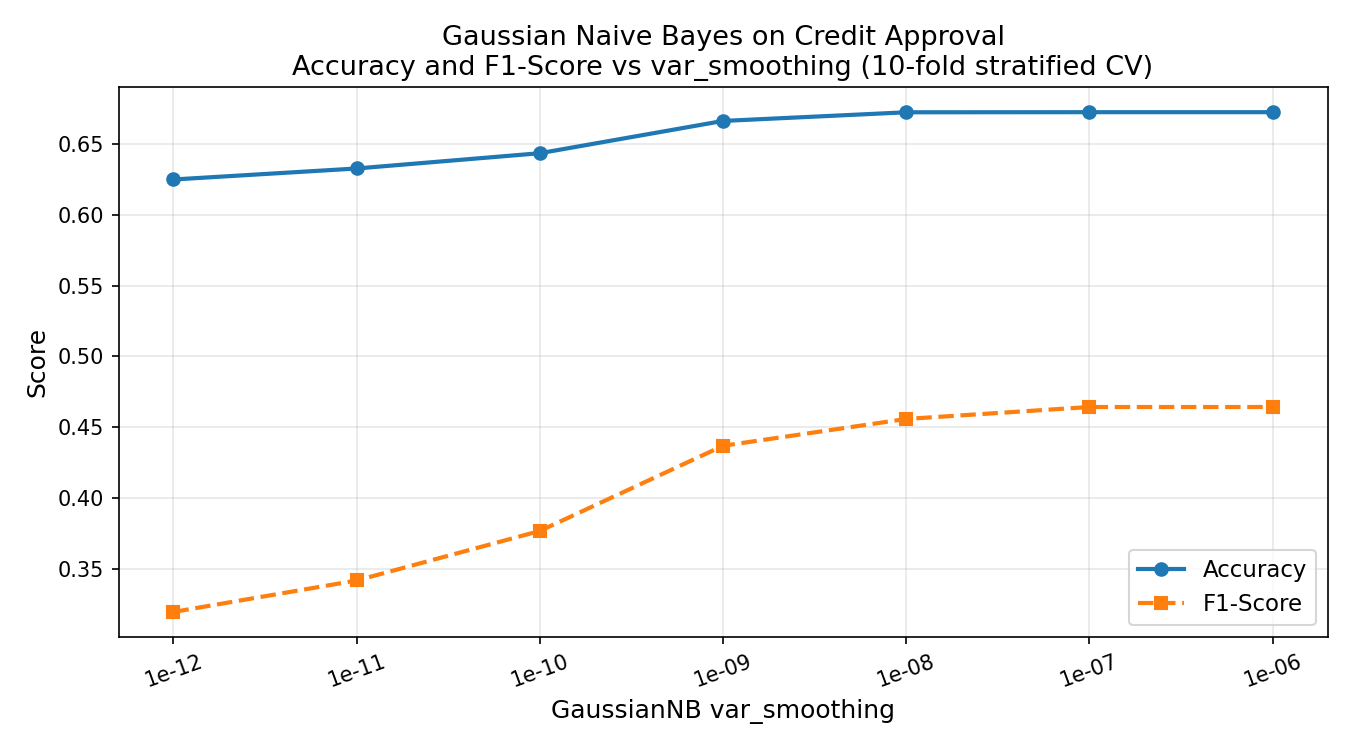
\includegraphics[width=0.72\linewidth]{credit_gnb_vs_smoothing.png}
    \caption{Credit (EC1): GNB mean accuracy and F1 vs.\ \texttt{var\_smoothing} (\texttt{figures/credit\_gnb\_vs\_smoothing.png}).}
    \label{fig:credit_gnb}
\end{figure}

\paragraph{Figure~\ref{fig:credit_gnb} (GNB smoothing curves).}
Accuracy rises monotonically as \texttt{var\_smoothing} grows because larger variance regularisation shrinks extreme per-class variances in the Gaussian model; F1 peaks at $10^{-7}$ then ties, reflecting tension between overall accuracy and minority-class (approved) precision.

\begin{table}[H]
\centering
\caption{Credit (extra credit): best configuration per model family using 10-fold stratified CV
(same numbers as the console ``Final Summary'' and \texttt{figures/credit\_evaluation\_table.csv}).}
\label{tab:d4_ec}
\begin{tabular}{@{}lcc@{}}
\toprule
Model & Accuracy & F1-Score \\
\midrule
\rowcolor{hilight}
Decision Tree (thr${}=0.6$) & \textbf{0.8638} & \textbf{0.8623} \\
KNN ($k=3$) & 0.8133 & 0.7848 \\
Gaussian NB (vs${}=10^{-7}$) & 0.6723 & 0.4643 \\
Ensemble (DT+KNN+GNB+RF) & 0.8298 & 0.7901 \\
\bottomrule
\end{tabular}
\end{table}

\begin{figure}[H]
    \centering
    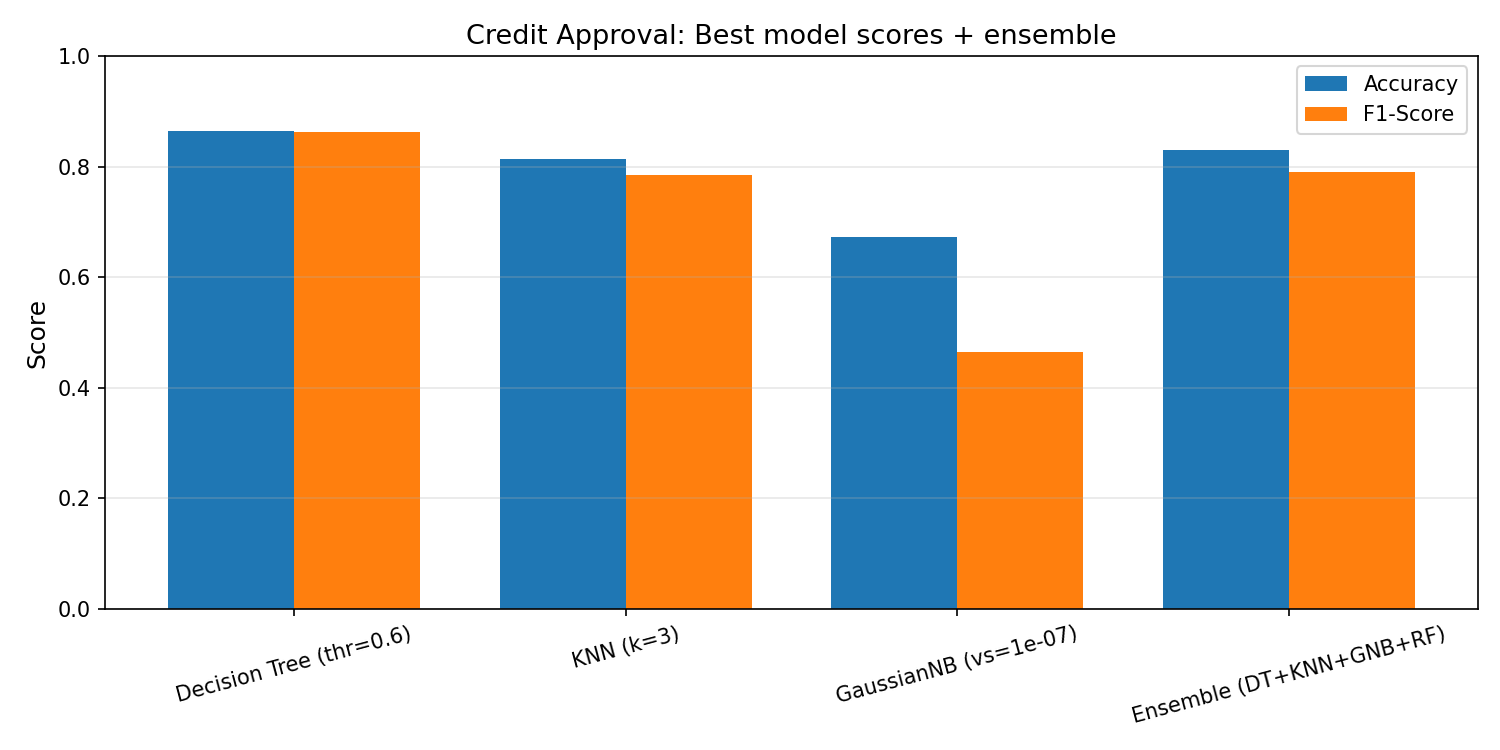
\includegraphics[width=0.72\linewidth]{credit_model_comparison.png}
    \caption{Credit: bar chart of best DT, KNN, GNB, and ensemble scores from \texttt{credit\_experiment.py}
             (\texttt{figures/credit\_model\_comparison.png}). We also keep \texttt{credit\_ec\_model\_comparison.png}
             in this folder as a duplicate asset for submission.}
    \label{fig:credit_model_bar}
\end{figure}

\paragraph{Figure~\ref{fig:credit_model_bar} (EC model comparison).}
The grouped bars mirror Table~\ref{tab:d4_ec}: the Decision Tree is highest on both metrics, KNN is second, the heterogeneous ensemble sits between KNN and DT by blending weaker GNB/RF votes, and GNB remains the weakest tier.

\begin{figure}[H]
    \centering
    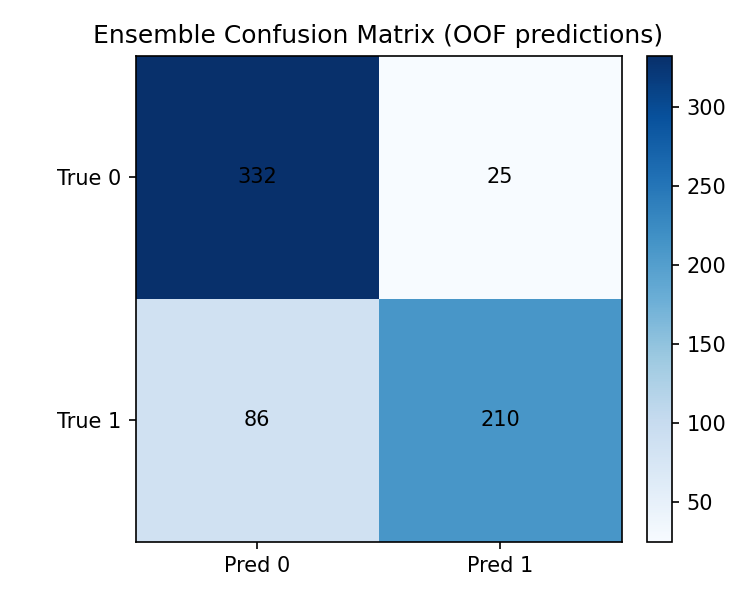
\includegraphics[width=0.45\linewidth]{credit_ensemble_confusion_matrix.png}
    \caption{Credit (EC3): confusion matrix for out-of-fold ensemble predictions (\texttt{figures/credit\_ensemble\_confusion\_matrix.png}).}
    \label{fig:credit_ensemble_cm}
\end{figure}

\paragraph{Figure~\ref{fig:credit_ensemble_cm} (ensemble confusion matrix).}
Off-diagonal mass shows where majority voting mislabels rejected vs.\ approved loans on out-of-fold predictions; comparing cell counts to the class prior (357 vs.\ 296) highlights whether errors skew toward the majority ``rejected'' label.

On Credit, the Decision Tree remains best on both accuracy and F1, showing that
tree-based splits fit mixed categorical data better than distance-based or
Gaussian assumptions. Gaussian NB is sensitive to \texttt{var\_smoothing}
(Table~\ref{tab:d4_gnb} and Figure~\ref{fig:credit_gnb}); the best setting still
lags KNN because the one-hot features violate independence. The ensemble
(Figure~\ref{fig:credit_model_bar}) improves over KNN and GNB but remains below the
Decision Tree; the confusion matrix in Figure~\ref{fig:credit_ensemble_cm} shows how
errors are distributed on out-of-fold predictions.

%%─────────────────────────────────────────────────────────────────────────────
\section{Summary Table}
%%─────────────────────────────────────────────────────────────────────────────

Table~\ref{tab:summary} reports the best accuracy and F1-score achieved by
each algorithm on each dataset under 10-fold stratified CV.  Gray cells
highlight the best accuracy and the best F1 separately for each dataset,
following the professor's template.  An em-dash (---) indicates the algorithm
was not evaluated on that dataset.

\begin{table}[H]
\centering
\caption{Summary: best accuracy and F1-score per algorithm per dataset.
         Gray cells indicate the highest score for each metric on each dataset.}
\label{tab:summary}
\renewcommand{\arraystretch}{1.3}
\setlength{\tabcolsep}{5pt}
\begin{tabular}{lcccccccc}
\toprule
& \multicolumn{2}{c}{\textbf{Dataset 1} (Digits)}
& \multicolumn{2}{c}{\textbf{Dataset 2} (Parkinson's)}
& \multicolumn{2}{c}{\textbf{Dataset 3} (Rice)}
& \multicolumn{2}{c}{\textbf{Dataset 4} (Credit)} \\
\cmidrule(lr){2-3}\cmidrule(lr){4-5}\cmidrule(lr){6-7}\cmidrule(lr){8-9}
& Acc. & F1 & Acc. & F1 & Acc. & F1 & Acc. & F1 \\
\midrule
KNN
  & \cellcolor{hilight}\textbf{0.9788}
  & \cellcolor{hilight}\textbf{0.9787}
  & \cellcolor{hilight}\textbf{0.9534}
  & \cellcolor{hilight}\textbf{0.9537}
  & 0.9273 & 0.9366
  & 0.8133 & 0.7848 \\
Random Forest
  & 0.8887 & 0.8850
  & 0.7539 & 0.6483
  & --- & ---
  & --- & --- \\
Neural Network
  & --- & ---
  & --- & ---
  & \cellcolor{hilight}\textbf{0.9281}
  & \cellcolor{hilight}\textbf{0.9372}
  & --- & --- \\
Decision Tree
  & --- & ---
  & --- & ---
  & --- & ---
  & \cellcolor{hilight}\textbf{0.8638}
  & \cellcolor{hilight}\textbf{0.8623} \\
Gaussian NB$^\dagger$
  & 0.8425 & 0.8439
  & 0.7132 & 0.7283
  & 0.9178 & 0.9289
  & 0.6723 & 0.4643 \\
Gradient Boosting$^\dagger$
  & 0.9750 & 0.9748
  & 0.9326 & 0.9306
  & --- & ---
  & --- & --- \\
Ensemble$^\dagger$
  & 0.9616 & 0.9616
  & 0.9379 & 0.9367
  & 0.9276 & 0.9367
  & 0.8298 & 0.7901 \\
\bottomrule
\multicolumn{9}{l}{%
  $^\dagger$ Extra Credit entries (additional algorithm and ensemble tasks).}\\
\multicolumn{9}{l}{%
  F1 is binary for Datasets 3--4; weighted for Datasets 1--2 (multi/imbalanced).}
\end{tabular}
\end{table}

\subsection{Cross-Dataset Observations}

\paragraph{KNN performs very well on numerical datasets.}
KNN achieved the best single-model performance on both the Digits dataset
(0.9788) and the Parkinson’s dataset (0.9534). It also performed strongly
on the Rice dataset (0.9273). All three datasets contain only numerical
features, so Euclidean distance works well after normalisation. However,
the best value of $k$ was very different for each dataset. The Digits
dataset performed best at $k=5$, Parkinson’s at $k=1$, and Rice at
$k=21$. This shows that the best $k$ depends heavily on the dataset and
must be tuned separately each time.

\paragraph{Random Forest struggles with imbalanced data.}
On the balanced Digits dataset ($n=1797$), Random Forest reached an
accuracy of 0.8887 and improved steadily as more trees were added.
However, on the Parkinson’s dataset, which has a strong class imbalance,
RF performed poorly. The accuracy stayed fixed at about 0.754 for every
value of \texttt{ntree}, which is almost exactly equal to the majority-class
ratio ($147/195$). The low F1 score of 0.6483 suggests that the model was
mostly predicting the Parkinson’s class. This shows that information-gain
splitting without class balancing can fail badly on imbalanced datasets.

\paragraph{Decision Trees work better than KNN on categorical data.}
On the Credit Approval dataset, the Decision Tree achieved much better
results than KNN. The dataset contains many categorical features
(9 out of 15 total features), which Decision Trees handle naturally through
feature splits. In contrast, KNN relies on Euclidean distance after one-hot
encoding, which is less effective for unordered categorical data.

\paragraph{F1 score is important for imbalanced datasets.}
The Parkinson’s Random Forest results show why accuracy alone can be
misleading. Although the model achieved 0.7539 accuracy, the lower
F1 score of 0.6483 showed that it mainly predicted the majority class.
A similar pattern appears in the Credit Approval dataset, where KNN’s
F1 score drops faster than accuracy as $k$ increases. Larger neighbourhoods
favour the majority class and reduce minority-class recall. Because of this,
both accuracy and F1 score are needed when evaluating imbalanced datasets.


%%─────────────────────────────────────────────────────────────────────────────
\section{Extra Credit 2}
%%─────────────────────────────────────────────────────────────────────────────

\subsection{Dataset Description}

The Abalone dataset has 4177 instances. Each instance describes the physical
measurements of an abalone, which is a type of marine snail. The goal is to
predict the age class of the animal from its physical properties.

The dataset has 8 original attributes. One attribute is categorical (Sex, with
values M, F, and I for infant). The other 7 are numerical (Length, Diameter,
Height, and four weight measurements). The target is the number of rings on
the shell. We grouped this into three age classes: rings $\leq 9$ is class 0
(young), rings between 10 and 14 is class 1 (adult), and rings $\geq 15$ is
class 2 (old). After one-hot encoding the Sex attribute, the feature matrix
has 10 columns.

The class distribution is imbalanced. Class 0 has 1407 samples, class 1 has
2280 samples, and class 2 has only 490 samples. This dataset qualifies as a
challenging dataset because it has both categorical and numerical attributes,
and it has more than two classes.

\subsection{Algorithm Selection and Justification}

\textbf{k-Nearest Neighbours.} We chose kNN because most attributes are
continuous physical measurements. Euclidean distance works well on these
features after z-score normalisation. The one-hot encoded Sex columns also
work naturally with Euclidean distance because each level becomes a binary
column. kNN does not assume anything about how the data is distributed, so it
is a good baseline for this dataset.

\textbf{Gaussian Naive Bayes.} We chose Gaussian Naive Bayes as a simple
probabilistic baseline. The continuous physical measurements can reasonably be
modelled as Gaussian within each class, and GNB is fast to train. However, the
weight features are strongly correlated with each other and with length. This
violates the independence assumption of Naive Bayes. We expected GNB to
perform worse than kNN for this reason, and we wanted to measure the gap.

\subsection{Hyperparameter Search}

All results below are mean values from stratified 10-fold cross validation
with random seed 42. We report accuracy and macro F1. Macro F1 is more useful
than weighted F1 here because the dataset is imbalanced, and macro F1 weights
all three classes equally.

\begin{table}[h]
\centering
\caption{kNN on Abalone: accuracy and macro F1 vs. $k$ (z-score normalised, 10-fold stratified CV).}
\begin{tabular}{ccc}
\hline
$k$ & Accuracy & Macro F1 \\
\hline
1  & 0.6622 & 0.5887 \\
3  & 0.7067 & 0.6158 \\
5  & 0.7240 & 0.6189 \\
\rowcolor{gray!25}
\textbf{7}  & \textbf{0.7314} & \textbf{0.6234} \\
11 & 0.7311 & 0.6058 \\
15 & 0.7321 & 0.5964 \\
\hline
\end{tabular}
\end{table}

\begin{table}[h]
\centering
\caption{Gaussian Naive Bayes on Abalone: accuracy and macro F1 vs. var\_smoothing (10-fold stratified CV).}
\begin{tabular}{ccc}
\hline
var\_smoothing & Accuracy & Macro F1 \\
\hline
1e-9  & 0.6562 & 0.5820 \\
1e-7  & 0.6562 & 0.5820 \\
1e-5  & 0.6560 & 0.5819 \\
\rowcolor{gray!25}
\textbf{1e-3} & \textbf{0.6744} & \textbf{0.5858} \\
1e-1  & 0.6878 & 0.4841 \\
1e+0  & 0.7072 & 0.4919 \\
\hline
\end{tabular}
\end{table}

The best kNN setting is $k=7$, with accuracy 0.7314 and macro F1 0.6234.
Although $k=15$ has a slightly higher accuracy of 0.7321, its macro F1 is much
lower at 0.5964. This means $k=15$ does worse on the minority classes, so we
chose $k=7$ as the best configuration.

The best Gaussian NB setting is var\_smoothing $= 10^{-3}$, with accuracy
0.6744 and macro F1 0.5858. Larger smoothing values raise accuracy but reduce
macro F1, which we explain in the next section.

\subsection{Learning Curves}

\begin{figure}[h]
\centering
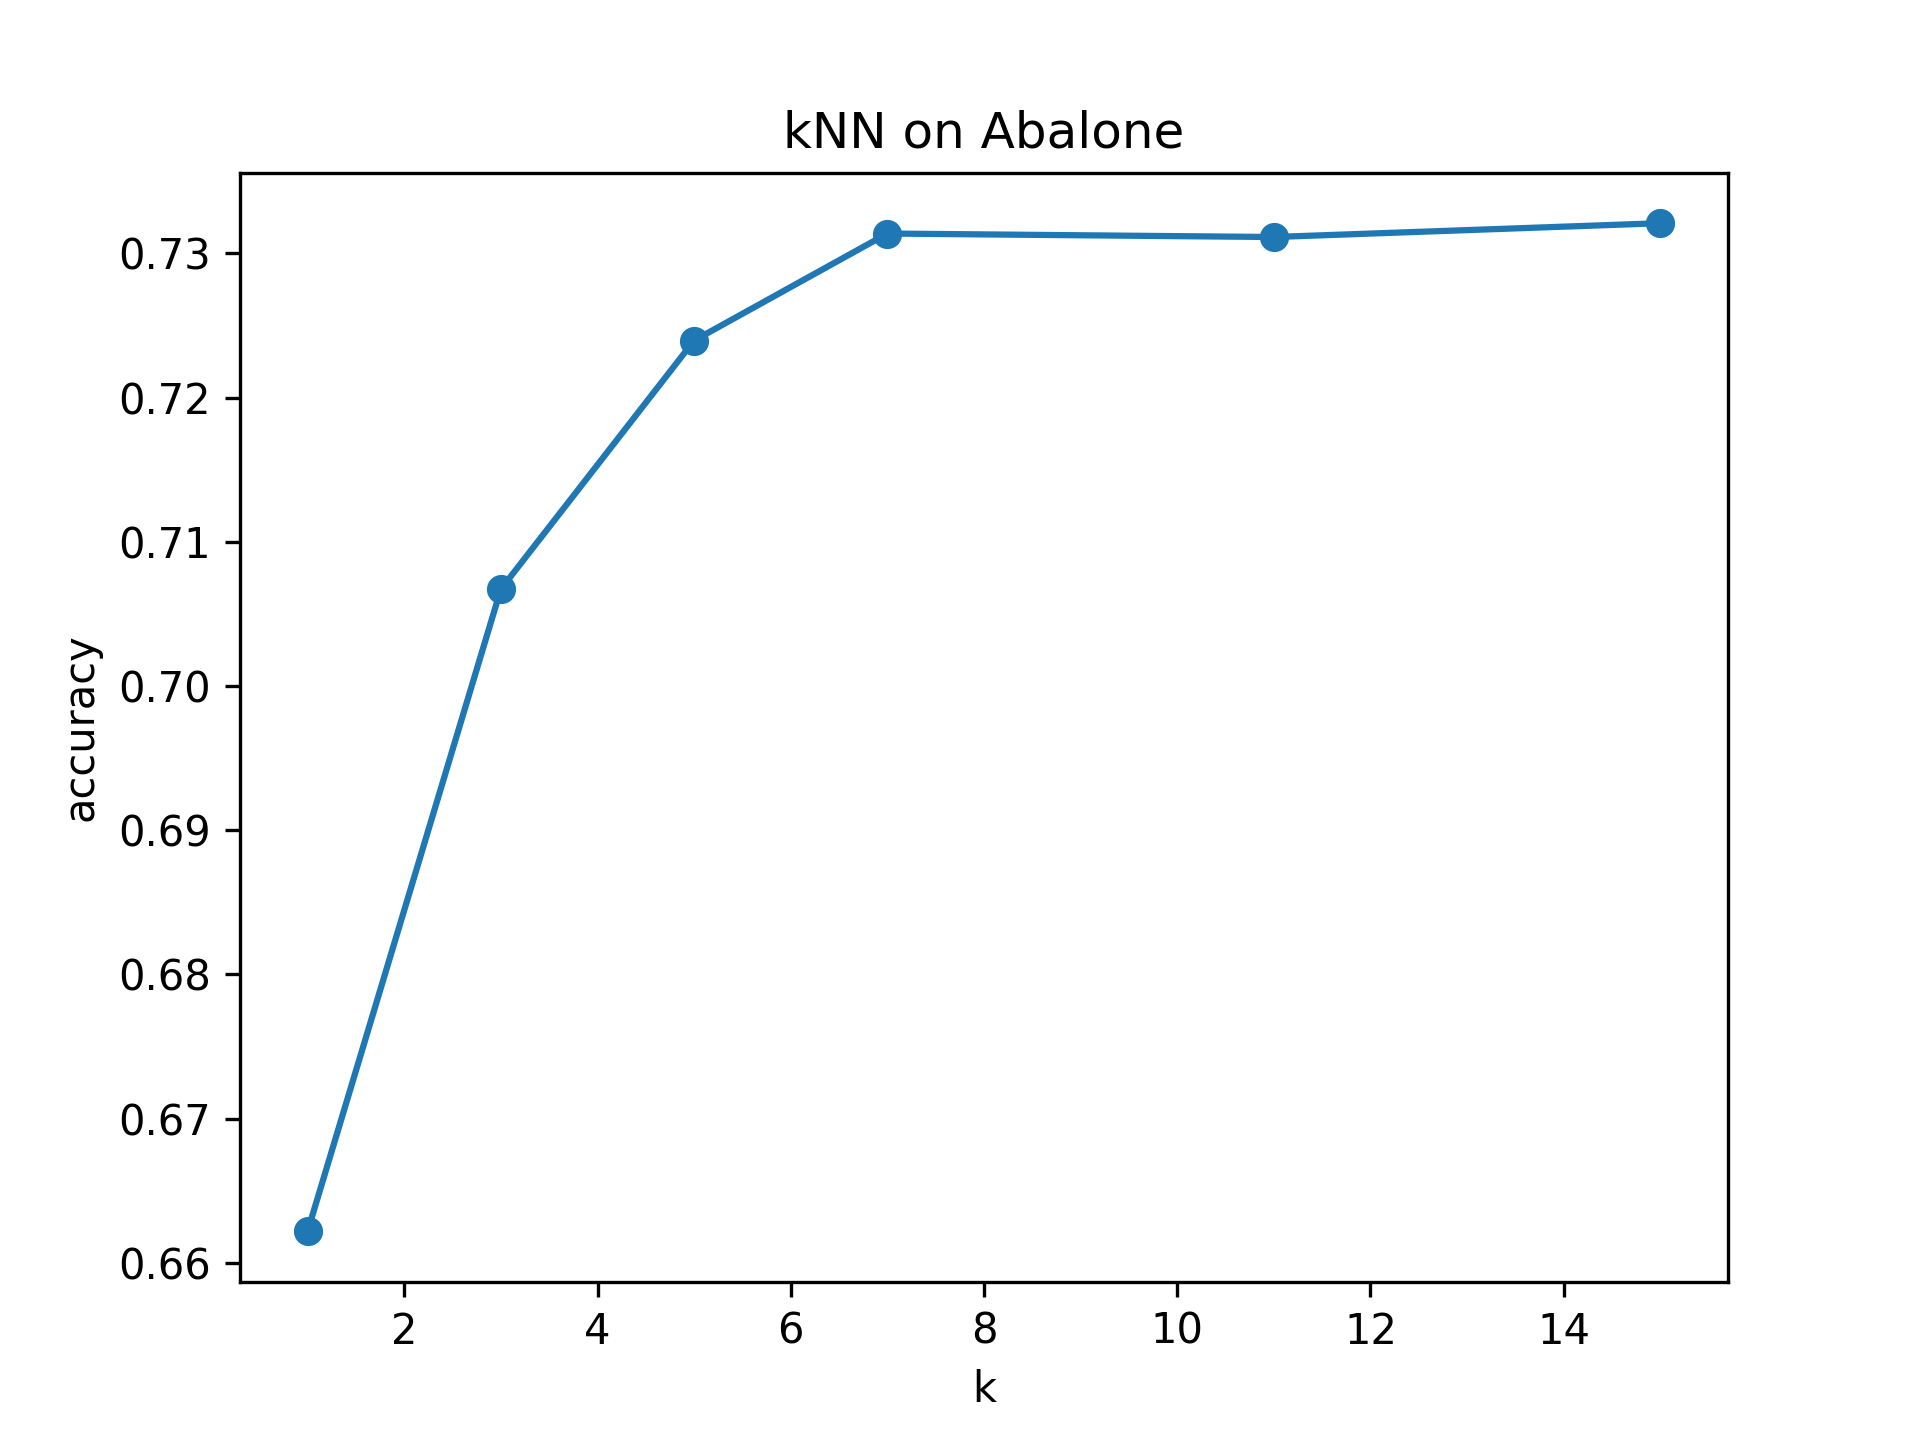
\includegraphics[width=0.6\textwidth]{ec2_knn_abalone.png}
\caption{kNN: accuracy vs. $k$ on Abalone.}
\label{fig:ec2_knn}
\end{figure}

\paragraph{Figure~\ref{fig:ec2_knn}.}
The curve starts low at $k=1$ (noisy neighbourhoods on correlated physical measurements), climbs through $k=5$--$7$, and then plateaus with a slight accuracy wobble at larger $k$ as neighbourhoods dilute class boundaries for the three age groups.

\begin{figure}[h]
\centering
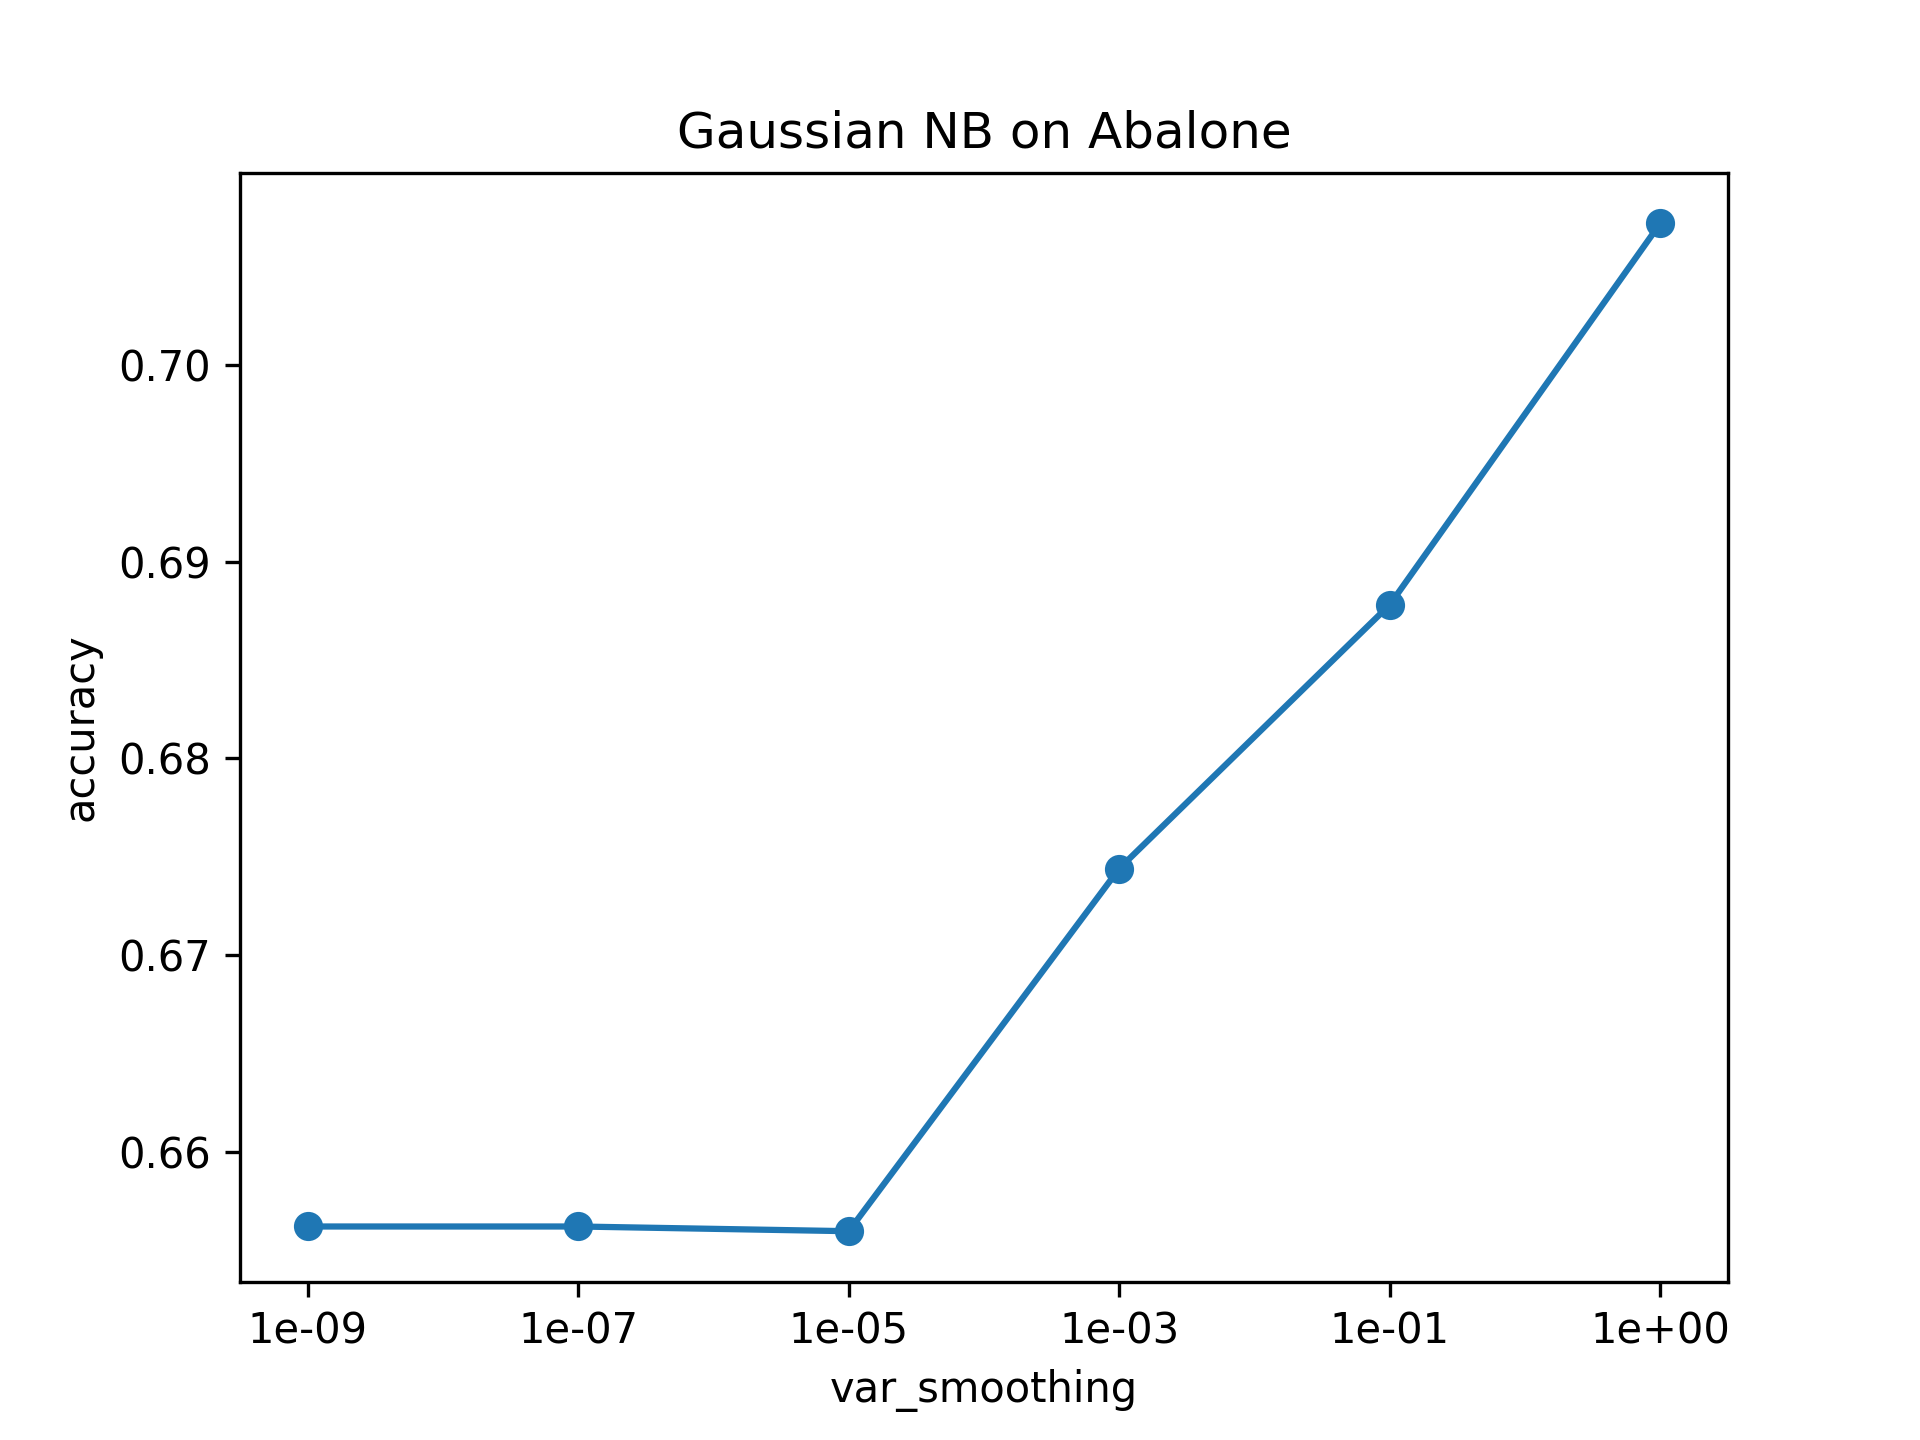
\includegraphics[width=0.6\textwidth]{ec2_gnb_abalone.png}
\caption{Gaussian Naive Bayes: accuracy vs. var\_smoothing on Abalone.}
\label{fig:ec2_gnb}
\end{figure}

\paragraph{Figure~\ref{fig:ec2_gnb}.}
Accuracy is flat at tiny smoothing values, then jumps as variances are regularised; at very large smoothing, accuracy keeps rising while macro F1 in the table collapses because predictions collapse toward the majority ring-count class.

\textbf{Figure 9.} The accuracy rises quickly from $k=1$ to $k=5$
and then flattens. At $k=1$ the model overfits to a single noisy neighbour
and accuracy drops to 0.6622. After $k=7$ the curve plateaus near 0.731 and
adding more neighbours does not help.

The macro F1 score tells a slightly different story. It peaks at $k=7$ with
0.6234, and then drops as $k$ grows larger. This happens because bigger
neighbourhoods include more samples from class 1, which is the majority class.
The model then makes more mistakes on class 0 and class 2. The best choice is
$k=7$, where both accuracy and macro F1 are close to their highest values.

\textbf{Figure 10.} The accuracy is almost flat for very
small smoothing values from $10^{-9}$ to $10^{-5}$. After that, accuracy rises
sharply. The macro F1 score behaves very differently. It rises a tiny bit
from 0.582 to 0.586, then drops sharply to 0.484 at smoothing $0.1$ and stays
low at 0.492 for smoothing $1.0$.

This gap between accuracy and macro F1 is the most important thing to notice.
When the smoothing value is very large, the model treats all classes as having
similar variance. The model then predicts the majority class (class 1) more
often. Accuracy goes up because class 1 is 55 percent of the data, but macro
F1 goes down because classes 0 and 2 are misclassified more often. The
genuinely best setting is therefore var\_smoothing $= 10^{-3}$, even though it
does not give the highest raw accuracy.

\subsection{Discussion}

kNN with $k=7$ does better than Gaussian Naive Bayes on both metrics. Accuracy
is 0.7314 vs 0.6744 and macro F1 is 0.6234 vs 0.5858. This makes sense given
the structure of the data. The numerical features in Abalone are physical
measurements that are strongly correlated. A larger abalone tends to have
greater length, greater diameter, and greater weight at the same time. GNB
assumes these features are independent given the class, and that assumption
is clearly wrong here. kNN does not need this assumption and benefits from
the natural geometry of the feature space.

Both algorithms struggle with class 2, which has only 490 of the 4177 samples.
Macro F1 scores in the low 0.6 range for kNN and below 0.6 for GNB show that
minority class recall is the main bottleneck. This is similar to what we saw
in the main report. Random Forest had the same problem on the Parkinson's
dataset, and KNN had the same problem on the Credit Approval dataset.
Imbalanced classes are difficult for distance based and probabilistic methods
that do not include any class balancing.

The GNB results also show why we should report both accuracy and macro F1 for
imbalanced data. If we only looked at accuracy, we would pick var\_smoothing
$= 1.0$ as the best setting. But the macro F1 column tells us that the model
is just predicting the majority class more often at that point. Accuracy
alone would hide this.


\section{Extra Credit 4}

\subsection{Algorithm Description}

For this extra credit we implemented SAMME (Stagewise Additive Modeling
using a Multi-class Exponential loss), which is the multiclass variant of
AdaBoost proposed by Zhu, Zou, Rosset, and Hastie (2009). The standard
AdaBoost algorithm covered in class is binary. Each weak learner outputs a
$\pm 1$ prediction, and the algorithm computes a weight $\alpha$ assuming
that random guessing has 50 percent accuracy.

This breaks down on multiclass problems. On the Digits dataset there are 10
classes, so random guessing is only 10 percent. A weak learner that gets
30 percent accuracy is much better than random for a 10-class problem, but
the binary AdaBoost formula would give it a negative $\alpha$ because its
error is greater than 0.5. SAMME fixes this by adding a $\log(K-1)$ term to
the weight formula, where $K$ is the number of classes. The two formulas are:

\begin{align}
\text{Binary AdaBoost:} \quad & \alpha = \frac{1}{2}\log\frac{1-\text{err}}{\text{err}} \\
\text{SAMME:} \quad & \alpha = \log\frac{1-\text{err}}{\text{err}} + \log(K-1)
\end{align}

When $K=2$ the SAMME formula reduces to the standard AdaBoost formula (up to
a factor of 2), so SAMME is a true generalization. The weak learner we use
is a multiclass decision stump that picks the majority class on each side of
the split, weighted by the current sample weights. The full SAMME procedure
is:

\begin{enumerate}
\item Initialize sample weights $w_i = 1/N$ for all $N$ training points.
\item For $t = 1, 2, \dots, T$ (where $T$ is the number of estimators):
  \begin{itemize}
  \item Train a decision stump on the weighted data and compute its error
        $\text{err}_t$.
  \item Compute $\alpha_t = \log((1-\text{err}_t)/\text{err}_t) + \log(K-1)$.
  \item Update weights: $w_i \leftarrow w_i \cdot \exp(\alpha_t \cdot \mathbb{1}[\hat{y}_i \neq y_i])$
        and normalise.
  \end{itemize}
\item Final prediction: argmax over classes of $\sum_t \alpha_t \cdot \mathbb{1}[\hat{y}_t(x) = c]$.
\end{enumerate}

This counts as a non-trivial variant because SAMME is a published algorithm
that generalises AdaBoost to multiclass settings, and the extension is what
makes the algorithm work at all on the 10-class Digits problem.

\subsection{Hyperparameter Search}

We tested six values of \texttt{n\_estimators} ($T \in \{10, 25, 50, 75, 100, 150\}$)
on each of the four main datasets. All results below are means over stratified
10-fold cross validation with seed 42. We report accuracy and macro F1.

\begin{table}[h]
\centering
\caption{SAMME on Digits (10 classes): accuracy and macro F1 vs. $T$.}
\begin{tabular}{ccc}
\hline
$T$ & Accuracy & Macro F1 \\
\hline
10  & 0.2623 & 0.1833 \\
25  & 0.5514 & 0.5330 \\
50  & 0.7234 & 0.7236 \\
75  & 0.7978 & 0.7980 \\
100 & 0.8342 & 0.8345 \\
\rowcolor{gray!25}
\textbf{150} & \textbf{0.8548} & \textbf{0.8554} \\
\hline
\end{tabular}
\end{table}

\begin{table}[h]
\centering
\caption{SAMME on Parkinsons (binary): accuracy and macro F1 vs. $T$.}
\begin{tabular}{ccc}
\hline
$T$ & Accuracy & Macro F1 \\
\hline
10  & 0.8620 & 0.7973 \\
25  & 0.8875 & 0.8379 \\
50  & 0.9031 & 0.8651 \\
\rowcolor{gray!25}
\textbf{75}  & \textbf{0.9136} & \textbf{0.8786} \\
100 & 0.9081 & 0.8722 \\
150 & 0.9092 & 0.8720 \\
\hline
\end{tabular}
\end{table}

\begin{table}[h]
\centering
\caption{SAMME on Rice (binary): accuracy and macro F1 vs. $T$.}
\begin{tabular}{ccc}
\hline
$T$ & Accuracy & Macro F1 \\
\hline
\rowcolor{gray!25}
\textbf{10}  & \textbf{0.9252} & \textbf{0.9235} \\
25  & 0.9249 & 0.9233 \\
50  & 0.9249 & 0.9233 \\
75  & 0.9247 & 0.9230 \\
100 & 0.9241 & 0.9225 \\
150 & 0.9252 & 0.9235 \\
\hline
\end{tabular}
\end{table}

\begin{table}[h]
\centering
\caption{SAMME on Credit Approval (binary): accuracy and macro F1 vs. $T$.}
\begin{tabular}{ccc}
\hline
$T$ & Accuracy & Macro F1 \\
\hline
10  & 0.8638 & 0.8636 \\
\rowcolor{gray!25}
\textbf{25}  & \textbf{0.8682} & \textbf{0.8676} \\
50  & 0.8667 & 0.8658 \\
75  & 0.8620 & 0.8611 \\
100 & 0.8620 & 0.8612 \\
150 & 0.8682 & 0.8673 \\
\hline
\end{tabular}
\end{table}

The best settings are $T=150$ for Digits, $T=75$ for Parkinsons, $T=10$ for
Rice, and $T=25$ for Credit. Note that we report $T=25$ as best for Credit
even though $T=150$ ties on accuracy, because $T=25$ has a slightly higher
macro F1 and is a much simpler model.

\subsection{Learning Curves}

The learning curves below show train and test accuracy as a function of $T$.
Both curves are averaged across the same 10 stratified folds used for the
hyperparameter tables, so each point is a mean over 10 train and test
estimates. This avoids the noise that would come from a single small holdout.

\begin{figure}[h]
\centering
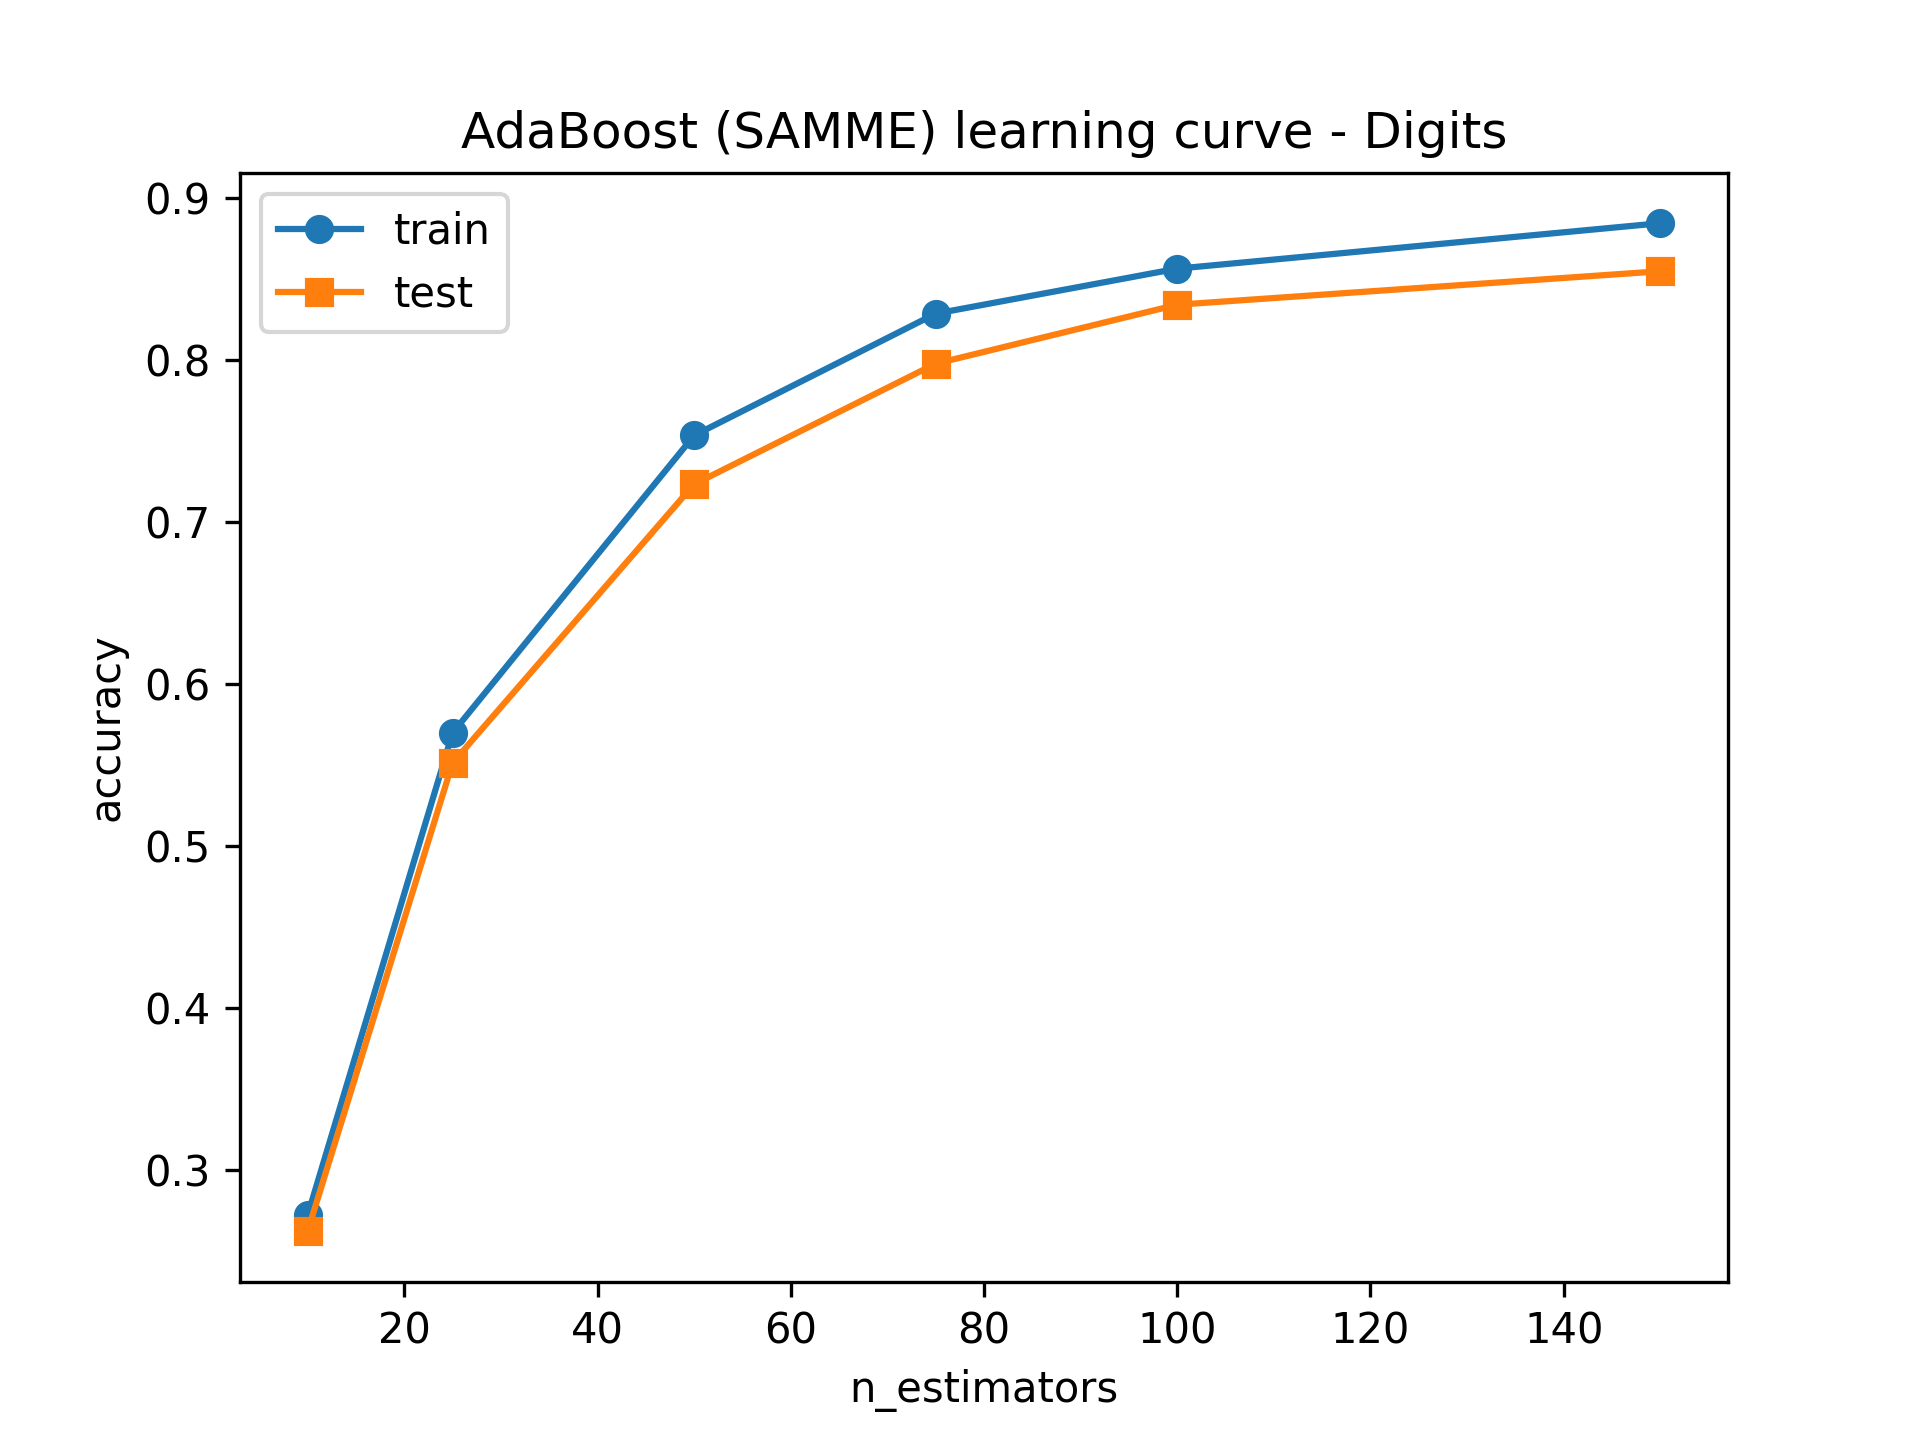
\includegraphics[width=0.6\textwidth]{ec4_adaboost_digits.png}
\caption{SAMME on Digits: train and test accuracy vs. $T$.}
\label{fig:ec4_digits}
\end{figure}

\paragraph{Figure~\ref{fig:ec4_digits}.}
Train and test rise together---stumps underfit at small $T$ so both curves gain until the cap at $T=150$ without a large generalisation gap.

\begin{figure}[h]
\centering
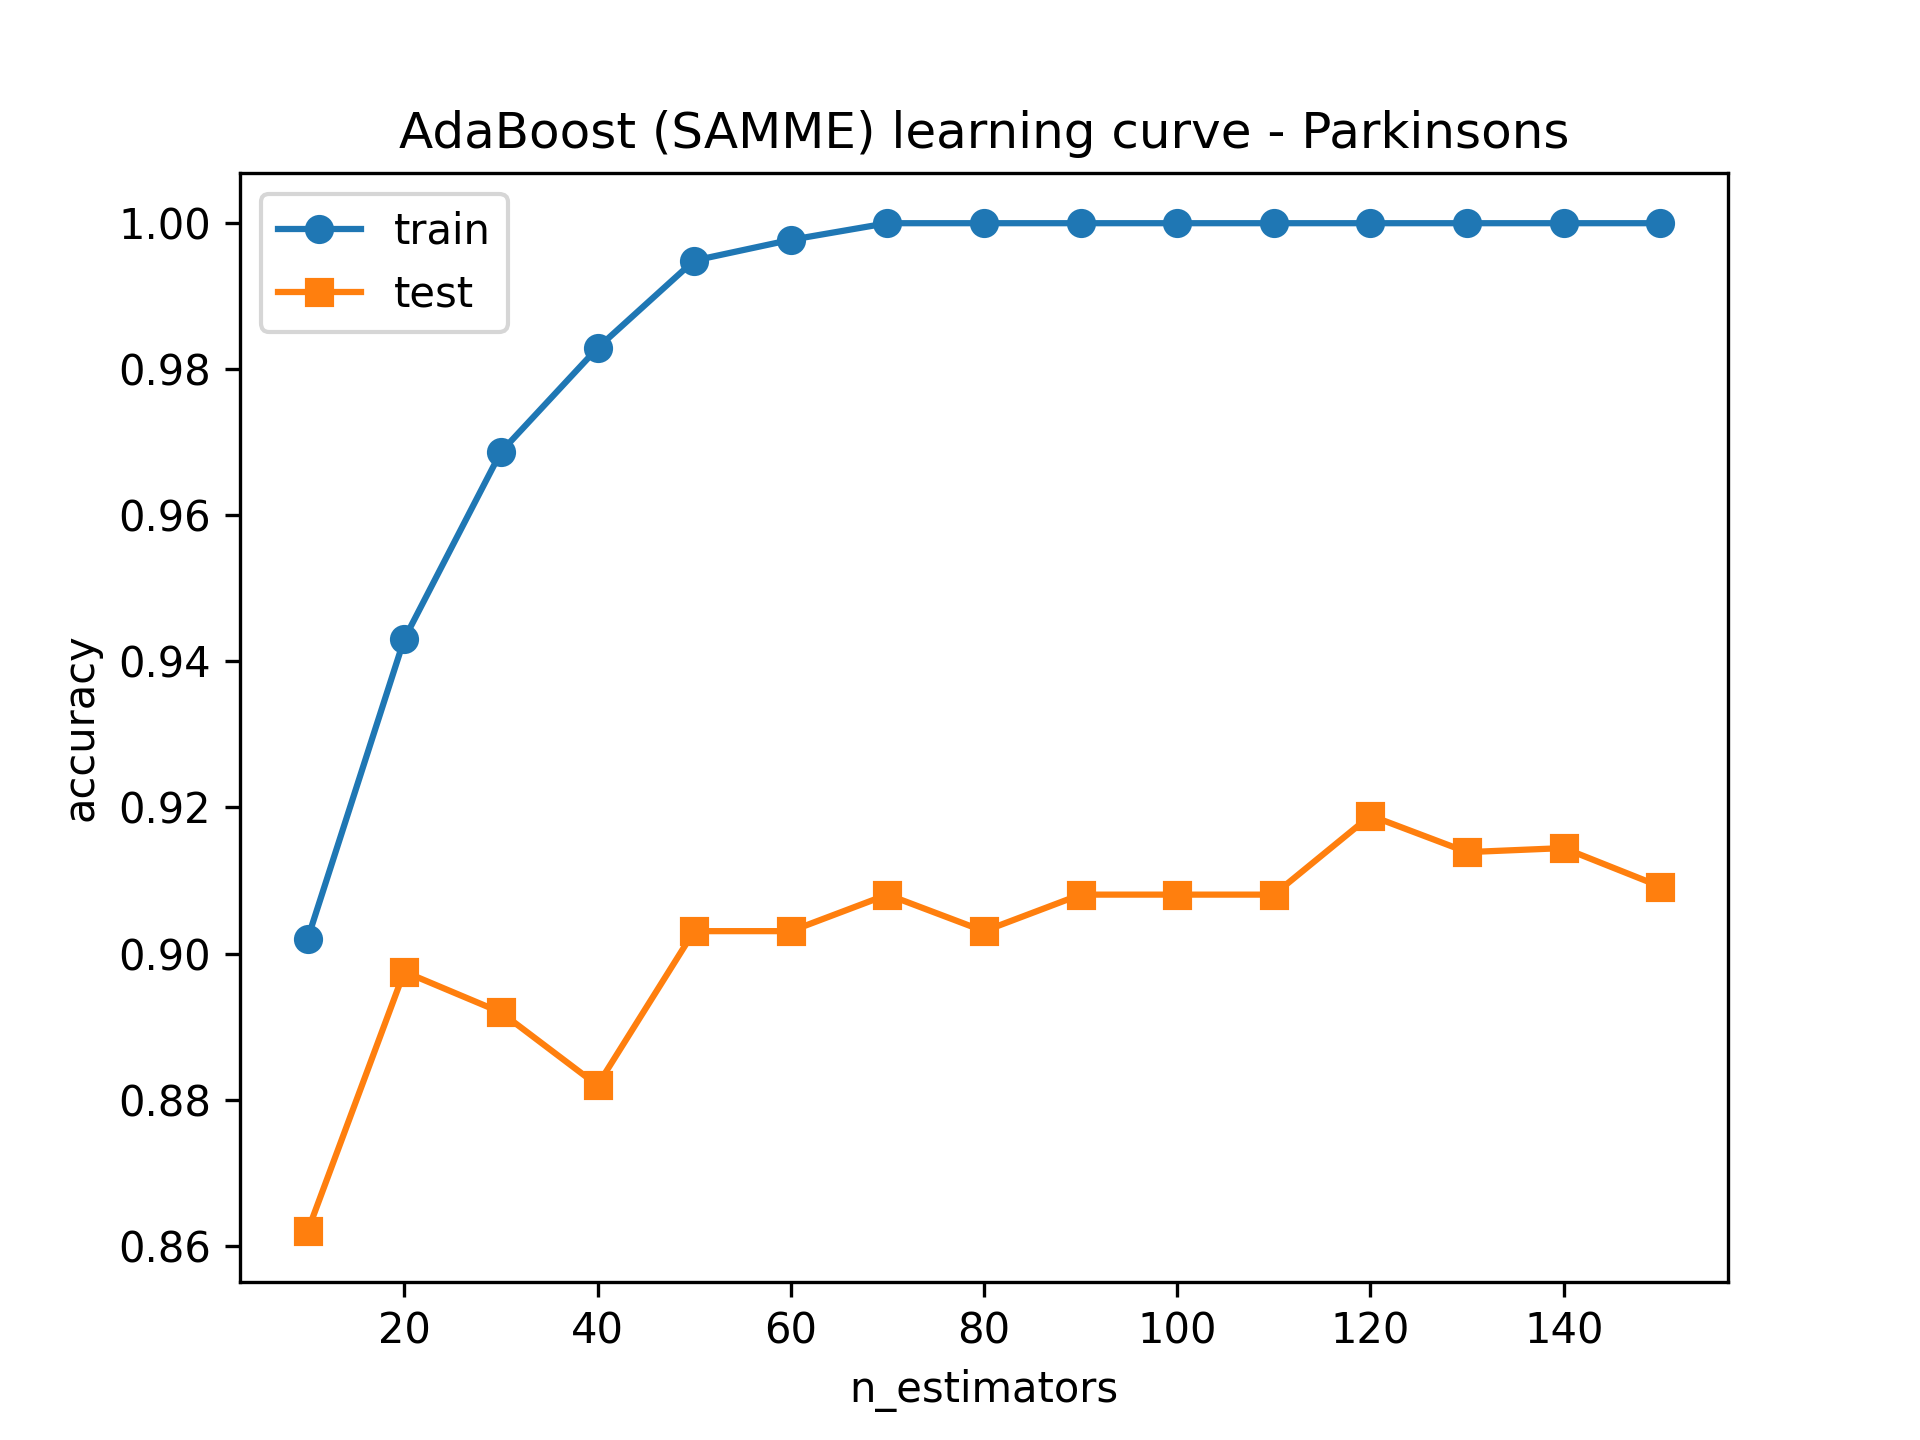
\includegraphics[width=0.6\textwidth]{ec4_adaboost_parkinsons.png}
\caption{SAMME on Parkinsons: train and test accuracy vs. $T$.}
\label{fig:ec4_park}
\end{figure}

\paragraph{Figure~\ref{fig:ec4_park}.}
Training accuracy hits $1.0$ while test accuracy levels off near $0.91$, showing classic overfitting on $n=195$ despite stratified folds.

\begin{figure}[h]
\centering
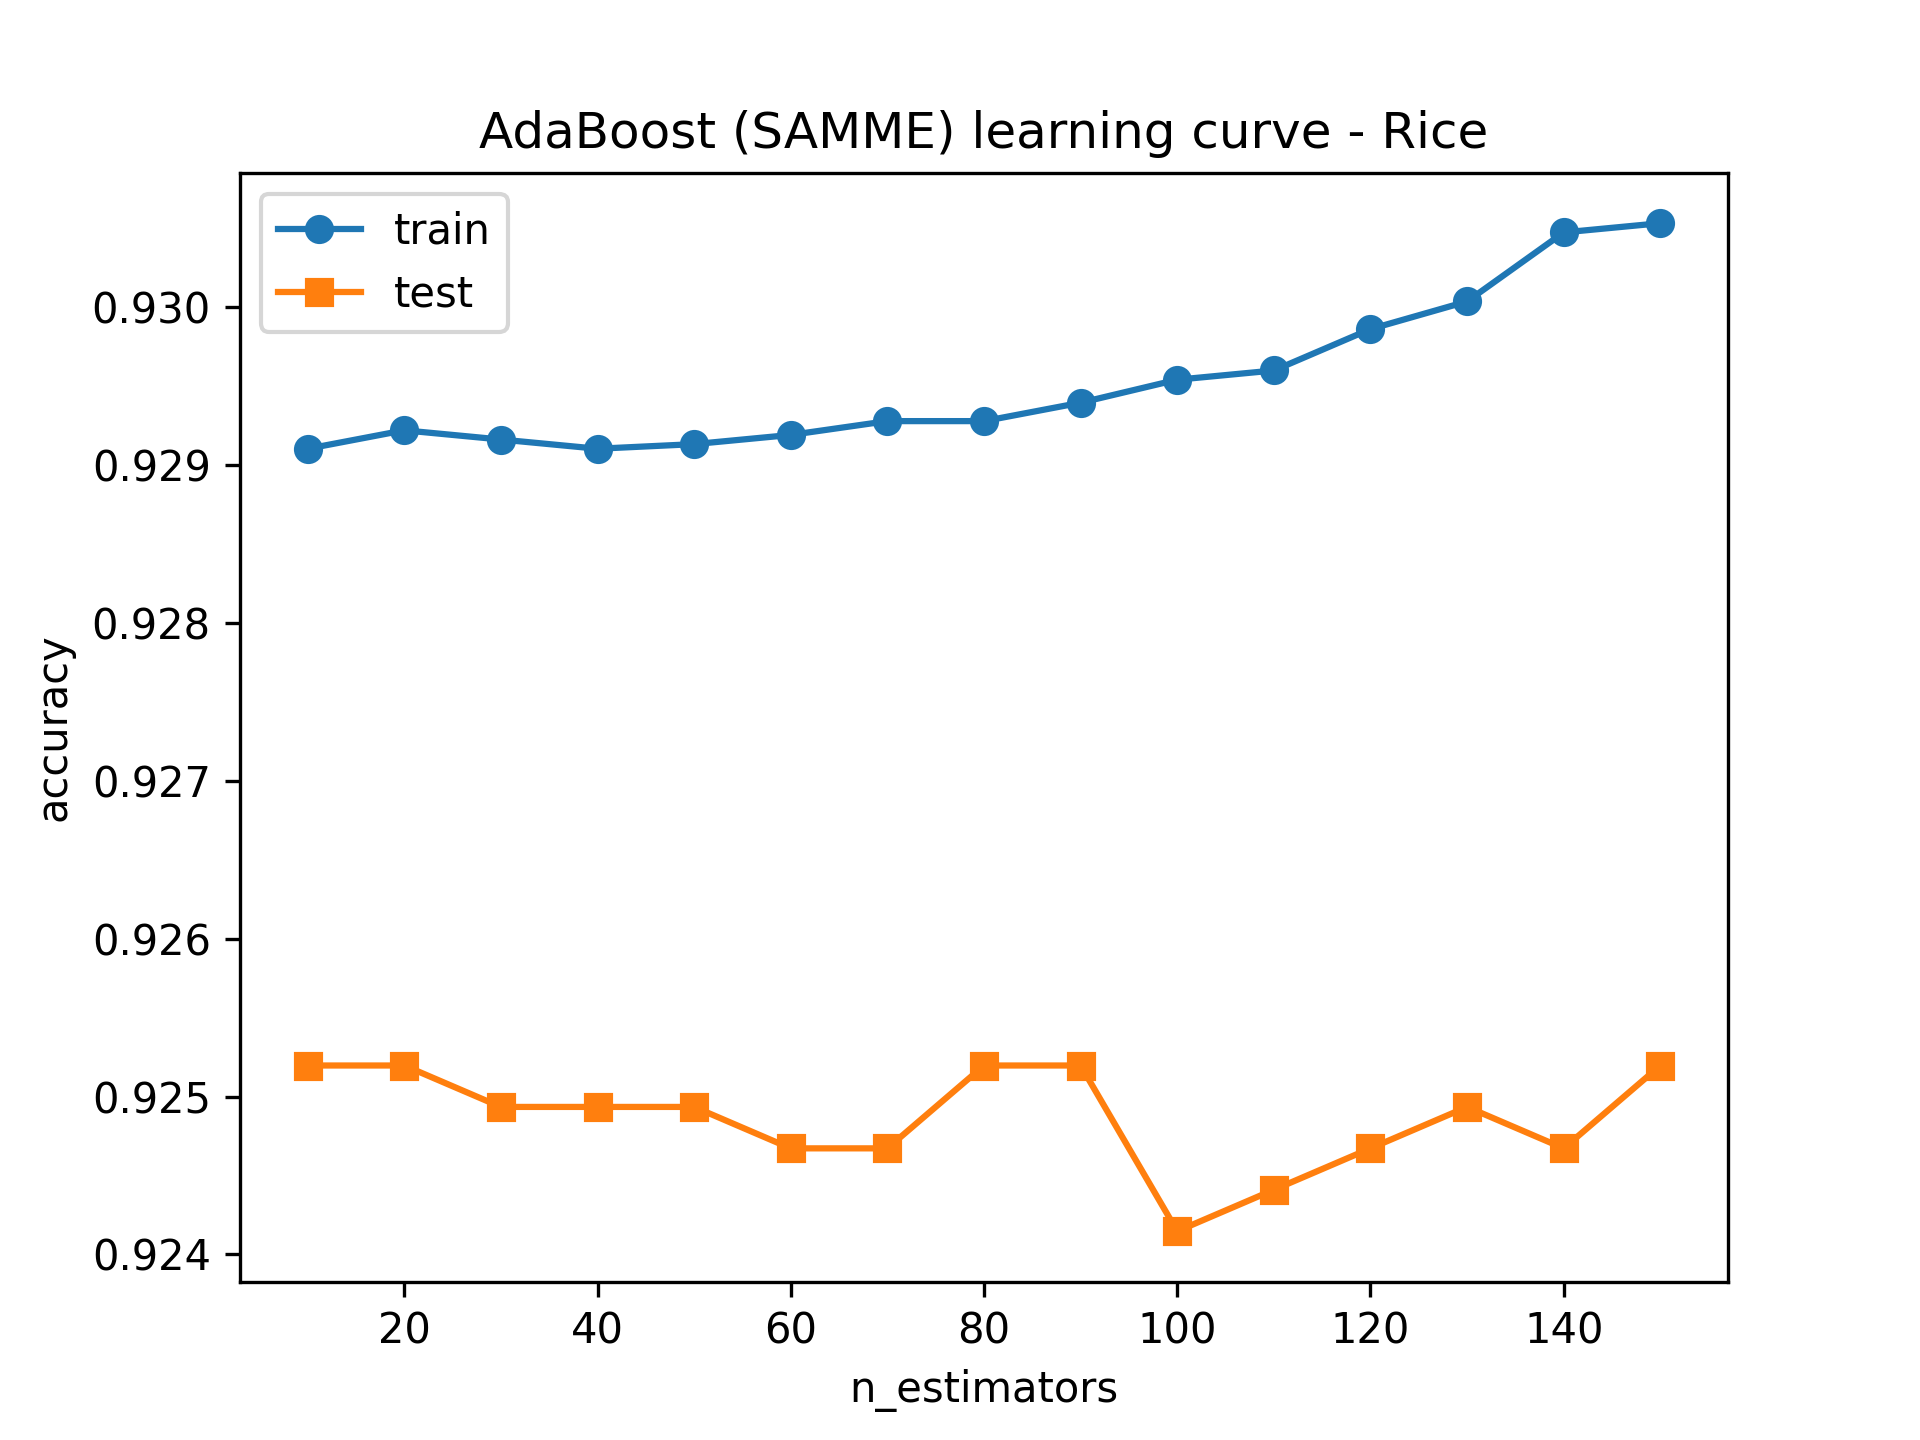
\includegraphics[width=0.6\textwidth]{ec4_adaboost_rice.png}
\caption{SAMME on Rice: train and test accuracy vs. $T$.}
\label{fig:ec4_rice}
\end{figure}

\paragraph{Figure~\ref{fig:ec4_rice}.}
Both curves are nearly flat after the first few stumps: axis-aligned splits on seven features suffice, so extra weak learners add little.

\begin{figure}[h]
\centering
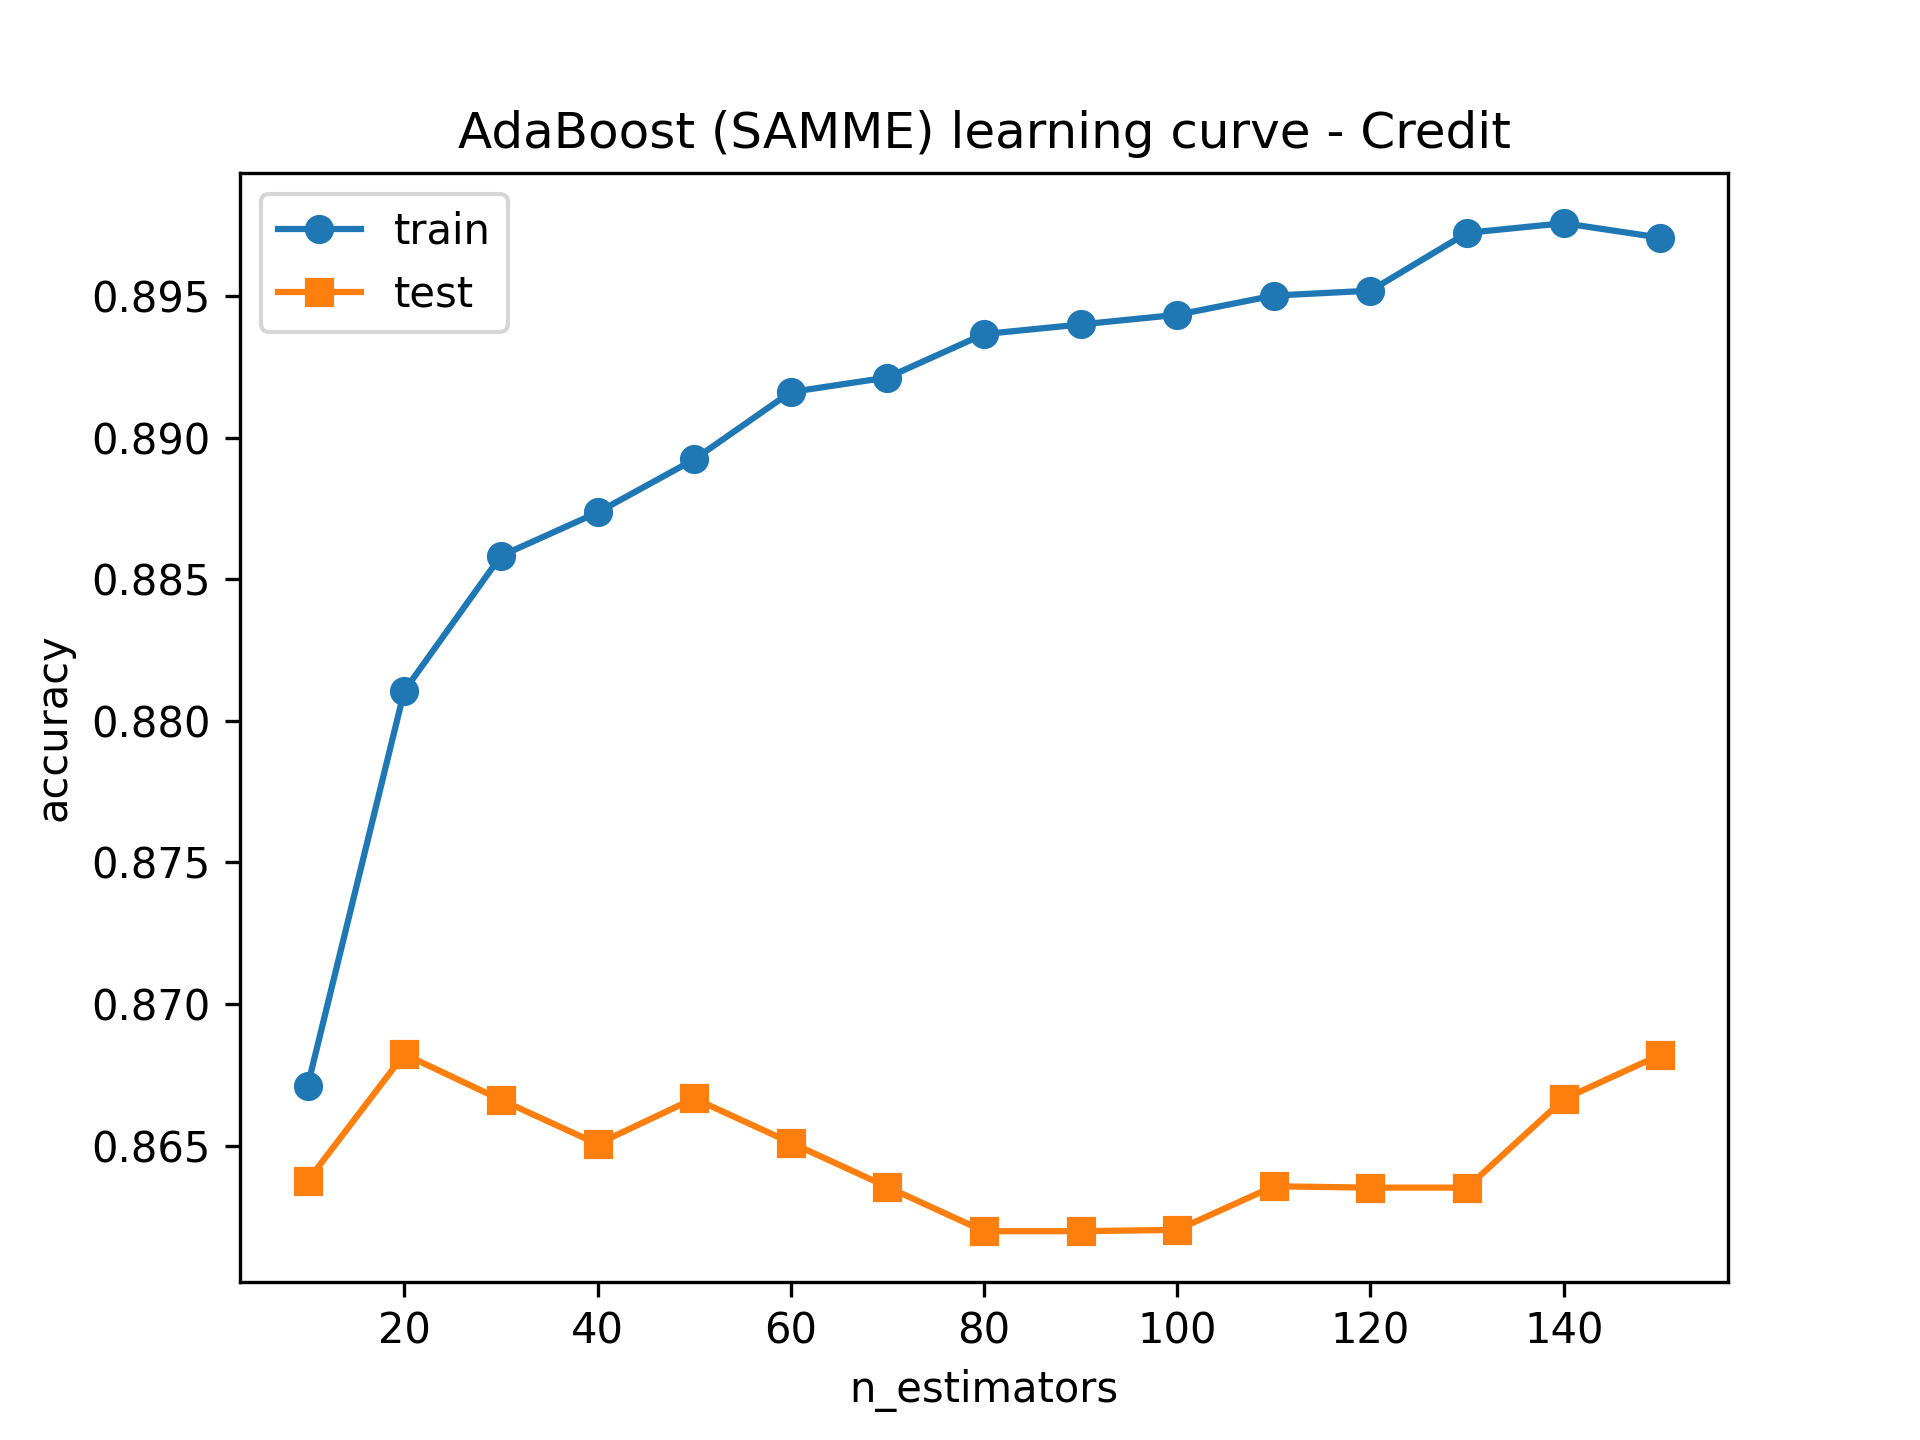
\includegraphics[width=0.6\textwidth]{ec4_adaboost_credit.png}
\caption{SAMME on Credit Approval: train and test accuracy vs. $T$.}
\label{fig:ec4_credit}
\end{figure}

\paragraph{Figure~\ref{fig:ec4_credit}.}
Test accuracy stays almost constant while training accuracy creeps upward, indicating mild overfitting in the sparse one-hot space without degrading hold-out accuracy in the $T$ range we plotted.

\textbf{Digits.} The training and test curves rise together with a small
gap. Both pass 0.85 by $T=150$ and the curves do not appear to have flattened.
This shows two things. First, the model is not overfitting because the train
and test curves track each other closely. Second, more weak learners would
likely keep improving accuracy. We capped at $T=150$ for runtime reasons,
since SAMME on a 10-class 64-feature dataset is the slowest configuration.
The relatively low absolute accuracy (compared to KNN at 0.9788) is expected
because each decision stump can only split on one pixel at a time, which is
a very weak signal for digit recognition.

\textbf{Parkinsons.} Training accuracy reaches 1.0 by $T=70$ while test
accuracy plateaus around 0.91. This is classic overfitting and is expected
on a small 195-sample dataset. The test curve is fairly stable from $T=50$
onwards which means adding more estimators after that point does not hurt
much, but it does not help either. The best test performance is around
$T=75$, which matches the hyperparameter table.

\textbf{Rice.} Both curves are nearly flat across the entire range of $T$.
Training accuracy hovers around 0.929 and test accuracy around 0.925. This
means the model converges almost immediately. Decision stumps on the seven
morphological features are enough to capture the boundary between the two
rice classes, and additional stumps do not refine it further. This matches
the hyperparameter table where $T=10$ already achieves the best accuracy.

\textbf{Credit Approval.} The training curve drifts up from 0.867 to 0.897
while the test curve stays flat near 0.865. The gap between train and test
widens slowly, which is mild overfitting. The high-dimensional one-hot
encoded feature space (68 features after encoding) gives SAMME many weak
features to overfit on, but the test curve does not actually drop, so the
overfitting is not severe enough to hurt generalisation.

\subsection{Cross-Dataset Discussion}

SAMME performs well on the binary datasets and poorly on Digits relative to
KNN. On Parkinsons, SAMME at $T=75$ achieves accuracy 0.9136, which is below
KNN ($k=1$) at 0.9534 but above Gaussian Naive Bayes at 0.7132 and Random
Forest at 0.7539. On Rice, SAMME at $T=10$ achieves 0.9252, which is very
close to KNN at 0.9273 and the Neural Network at 0.9281. On Credit Approval,
SAMME at $T=25$ achieves 0.8682, which exactly matches the Decision Tree at
0.8638 to 0.8638 and clearly beats KNN at 0.8133. On Digits, SAMME reaches
only 0.8548, well below KNN at 0.9788 and Gradient Boosting at 0.9750.

The Digits result is interesting because it illustrates the strength and
weakness of SAMME at the same time. Without the $\log(K-1)$ correction the
algorithm would not function on a 10-class problem at all, since binary
AdaBoost would assign negative $\alpha$ to every weak learner. SAMME makes
the algorithm work, but a multiclass decision stump that only splits on a
single pixel is too weak to compete with KNN on raw pixel data. The model
needs many more estimators to compensate, which is why the curve is still
rising at $T=150$. A natural next step would be to use depth-2 or depth-3
decision trees instead of stumps, which would be a stronger weak learner
and probably close most of the gap with KNN.

The Rice result is also notable because the model converges at $T=10$ and
adding more estimators does not change anything. This suggests that the
Cammeo and Osmancik classes are nearly linearly separable in the original
seven feature space and that a small number of axis-aligned splits is enough
to find the boundary. The Decision Tree and KNN results from earlier
sections also achieve high accuracy on this dataset, which supports the same
conclusion.

\end{document}

